\documentclass[aspectratio=169]{beamer}
\usetheme{SimpleDarkBlue}
\usecolortheme{default}
% \usefonttheme{serif}
\usepackage{helvet}
\usepackage[dvipsnames]{xcolor}
\usepackage{tabularx}
\usepackage{booktabs}
\usepackage[utf8]{inputenc}
\usepackage{longtable}
\usepackage{siunitx}
\usepackage{array, multirow, tabularx,tabu}

\usepackage[T1]{fontenc}
\usepackage{booktabs}
\usepackage{graphicx}

\usepackage{wrapfig}
\graphicspath{ {res/}{res/figures} }

\usepackage{amsmath,amssymb}

\usepackage{mathtools}
\usepackage{tikz}
\usepackage{hyperref}
\usepackage{multicol}
\usepackage{appendixnumberbeamer}
\usepackage{tikz}
\usetikzlibrary{calc, positioning, arrows.meta, arrows, shapes.geometric, shapes, backgrounds, overlay-beamer-styles}
\usetikzlibrary{decorations.pathreplacing,patterns}
\usepackage[
    natbib=true,
    style=numeric,
    sorting=none,
    maxcitenames=1,
    % style=authoryear
]{biblatex} 
\AtBeginBibliography{\tiny}

\addbibresource{res/biblio.bib} 
\addbibresource{res/biblio2.bib} 

\def\mrglu{\text{MR}_{\text{glu}}}
\newcommand{\fdg}{$[^{18}\mathrm{F}]\text{FDG}$}
\newcommand{\yohimbine}{$[^{11}\mathrm{C}]\text{Yohimbine}$}

\newcommand{\sym}[1]{\textsuperscript{#1}}

\makeatletter
\newcommand\titlegraphicii[1]{\def\inserttitlegraphicii{#1}}
\newcommand\titlegraphiciii[1]{\def\inserttitlegraphiciii{#1}}
\newcommand{\citeauthoryear}[1]{\citeauthor{#1} (\citeyear{#1})}


\newcounter{backupframe}
\newcommand{\backupfootline}{%
  \hfill\usebeamerfont{page number in head/foot}\usebeamercolor[fg]{page number in head/foot}%
  \roman{backupframe}\kern1em\vskip2pt%
}

% Environment to create a backup (noframenumbering) frame that shows Roman numerals
\newenvironment{backup}[1][]{%
  \stepcounter{backupframe}% increment backup counter
  \setbeamertemplate{footline}{\backupfootline}% install backup footline
  \begin{frame}[noframenumbering,#1]%
}{%
  \end{frame}%
  \setbeamertemplate{footline}[frame number]% restore main footline
}


\tikzset{
	invisible/.style={opacity=0,text opacity=0},
	visible on/.style={alt=#1{}{invisible}},
	alt/.code args={<#1>#2#3}{%
			\alt<#1>{\pgfkeysalso{#2}}{\pgfkeysalso{#3}} % \pgfkeysalso doesn't change the path
		},
}

\AtBeginSection[]{
  \begin{frame}
  \vfill
  \centering
  \begin{beamercolorbox}[sep=8pt,center,shadow=true,rounded=true]{title}
    \usebeamerfont{title}\insertsectionhead\par%
  \end{beamercolorbox}
  \vfill
  \end{frame}
}

\setbeamertemplate{footline}[frame number]{}
\setbeamertemplate{title page}
{
	\vbox{}
	{\usebeamercolor[fg]{titlegraphic}\inserttitlegraphic\inserttitlegraphiciii\hfill\inserttitlegraphicii\par}
	\begin{centering}
		\begin{beamercolorbox}[sep=8pt,center]{institute}
			\usebeamerfont{institute}\insertinstitute
		\end{beamercolorbox}
		\begin{beamercolorbox}[sep=8pt,center]{title}
			\usebeamerfont{title}\inserttitle\par%
			\ifx\insertsubtitle\@empty%
			\else%
				\vskip0.25em%
				{\usebeamerfont{subtitle}\usebeamercolor[fg]{subtitle}\insertsubtitle\par}%
			\fi%     
		\end{beamercolorbox}
		\vskip1em\par
		\begin{beamercolorbox}[sep=8pt,center]{date}
			\usebeamerfont{date}\insertdate
		\end{beamercolorbox}%\vskip0.5em
		\begin{beamercolorbox}[sep=8pt,center]{author}
			\usebeamerfont{author}\insertauthor
		\end{beamercolorbox}
	\end{centering}
	%\vfill
}
\makeatother

\title{Estimation of Image-Derived Input Function in Hybrid MRI and Dynamic Brain PET Imaging}
\author{Sepand Ali Madad Soltani\\ \vspace{0.5em} \tiny{Supervised by Dr. Nicolas Costes \& Dr. Inés Merida \\ \vspace{0.5em} Hosting Laboratory: CERMEP-Imagerie du Vivant, Lyon, France}}
\subtitle{Application to Modeling PET Dynamics of Glucose Metabolism in Patients with Impaired Consciousness}
\institute{\small Medical Device Engineering}
\institute{University of Claude Bernard Lyon 1-Polytech Lyon}

\date{September, 4 2025}
\titlegraphiciii{
\includegraphics[height=1cm]{polytech.png}}
\titlegraphic{
\includegraphics[height=1cm]{ucbl.png}}
\titlegraphicii{
\includegraphics[height=1cm]{cermep.png}}

\begin{document}

\begin{frame}[plain]
	\maketitle
	\small
	\centering
	\footnotesize
\end{frame}

\usetikzlibrary{positioning, arrows.meta}

% Define colors for outcomes
\definecolor{colAwake}{RGB}{0,153,51}
\definecolor{colNon}{RGB}{255,153,0}
\definecolor{colDeath}{RGB}{204,0,0}



\begin{frame}[t]{Positron Emission Tomography (PET)}
	\begin{columns}
		\begin{column}{0.7\textwidth}
			\begin{itemize}
				\setlength\itemsep{2em}
				\small
				\item In vivo functional imaging technique
				\item Intravenous injection of radioactive tracers
				\item Provides insight in physiological and biochemical processes
				\item Applications in oncology, neurology, drug development, etc.


				\item \textbf{Static PET:} Single-volume, semi-quantitative,\\ commonly used in \textbf{clinical} applications
				\item \textbf{Dynamic PET:} Multi-volume, absolute quantification, commonly used in \textbf{research} applications


			\end{itemize}
		\end{column}
		\begin{column}{0.25\textwidth}
			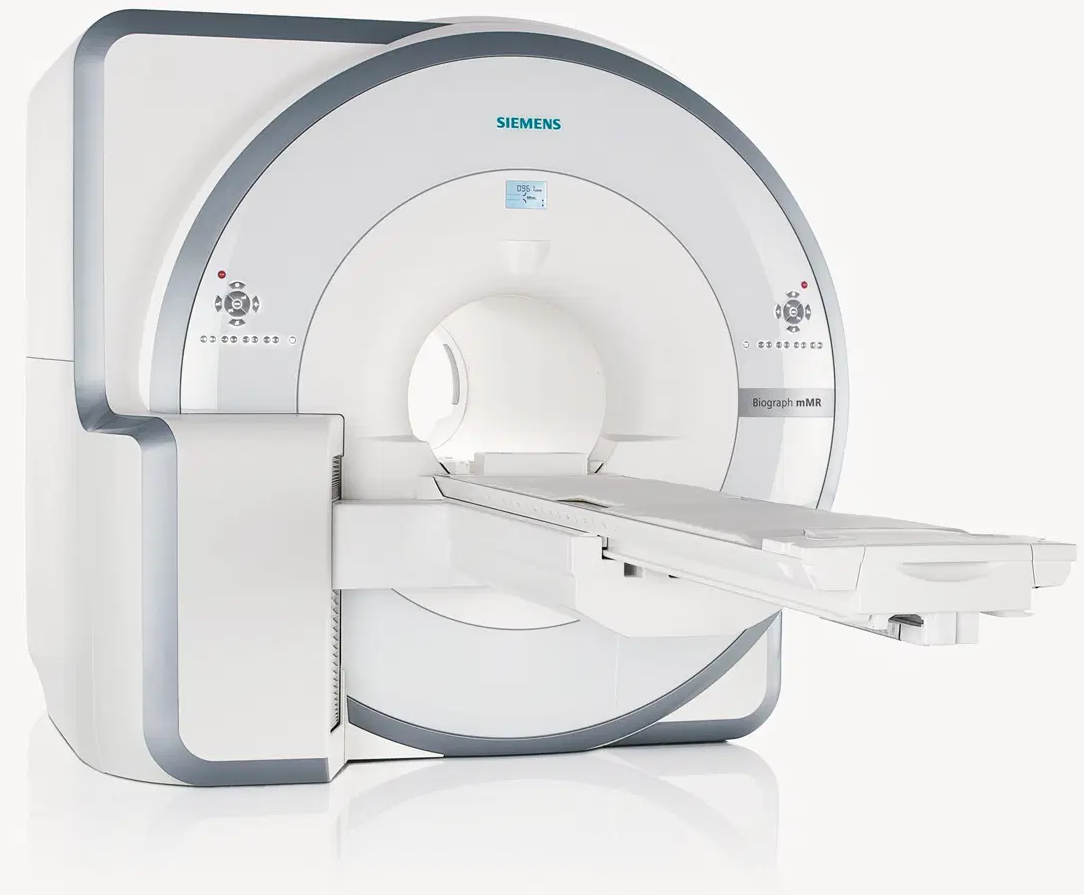
\includegraphics[width=\linewidth]{pet_machine2.png} \\ [0.5cm]
			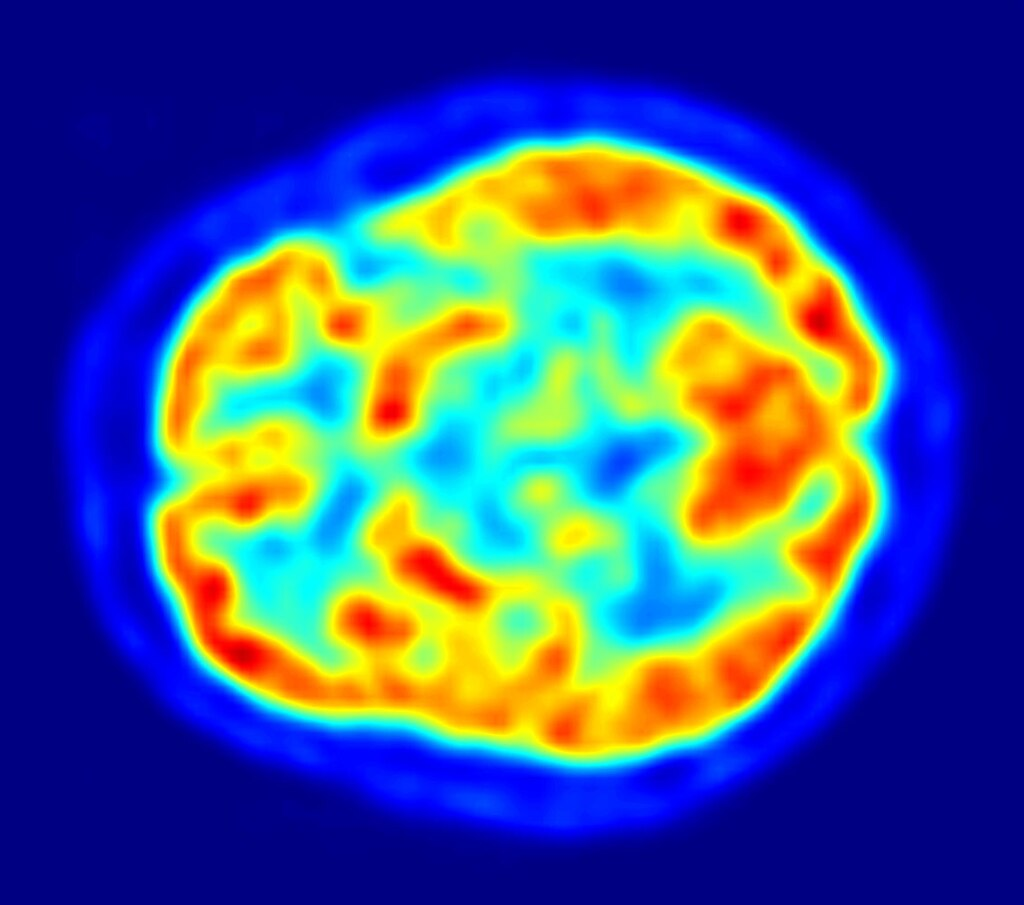
\includegraphics[width=\linewidth]{pet_image.jpg}
		\end{column}
	\end{columns}

\end{frame}

\begin{frame}[t]{Absolute Quantification in Dynamic PET}

	\begin{itemize}
		\item \textbf {Compartmental Model:} Allows for calculation of quantitative values ($\mrglu, V_T,\dots$)
	\end{itemize}
	\pause
	\centering
	\vspace{1em}
	\begin{tikzpicture}[>=latex, thick,node distance=1.5cm, decorate]
		\node[cylinder, draw, shape border rotate=90, aspect=0.3,
			minimum height=3cm, minimum width=1.7cm,
			align=center, fill=red!80] (Cp) at (0,0) {\small Input \\ Function};

		\node[draw, rounded corners, minimum width=2.5cm, minimum height=2cm, align=center] (C1) at (4,0) {Free tracer};
		\node[draw, rounded corners, minimum width=2.5cm, minimum height=2cm, align=center] (C2) at (8,0) {Bound tracer};

		\draw[->] ([yshift=8pt]Cp.east) to[out=0, in=180] ([yshift=8pt]C1.west);
		\draw[->] ([yshift=-8pt]C1.west) to[out=180, in=0] ([yshift=-8pt]Cp.east);
		\draw[->] ([yshift=8pt]C1.east) to[out=0, in=180] ([yshift=8pt]C2.west);
		\draw[->] ([yshift=-8pt]C2.west) to[out=180, in=0] ([yshift=-8pt]C1.east);

		\begin{pgfonlayer}{background}
			\coordinate (BoxTL) at ($(C1.north west)+(-0.3,0.3)$);
			\coordinate (BoxTR) at ($(C2.north east)+(0.3,0.3)$);
			\coordinate (BoxBR) at ($(C2.south east)+(0.3,-0.3)$);
			\coordinate (BoxBL) at ($(C1.south west)+(-0.3,-0.3)$);
			\draw[dashed, rounded corners, thick, fill=yellow!40] (BoxTL) rectangle (BoxBR);
		\end{pgfonlayer}

		\node at ($(Cp.north)+(0,0.3)$) {\textbf{Blood}};
		\node at ($($(BoxTL)!0.5!(BoxTR)$)+(0,0.3)$) {\textbf{Tissue}};

		\draw[decorate,visible on=<4->, decoration={brace, mirror, amplitude=5pt,raise=0.9cm}]
		(Cp.south west) -- node[below=1.5cm] {\scalebox{2}{\Huge\color{red}{?}}} (Cp.south east);

		\draw[decorate, visible on=<3->, decoration={brace, mirror, amplitude=5pt,raise=0.5cm}]
		(BoxBL) -- node[below=1cm] {} (BoxBR);


		\begin{scope}[yshift=-5cm,visible on=<3->]
			\node at ($($(BoxBL)!0.5!(BoxBR)$)+( 0, -2)$) {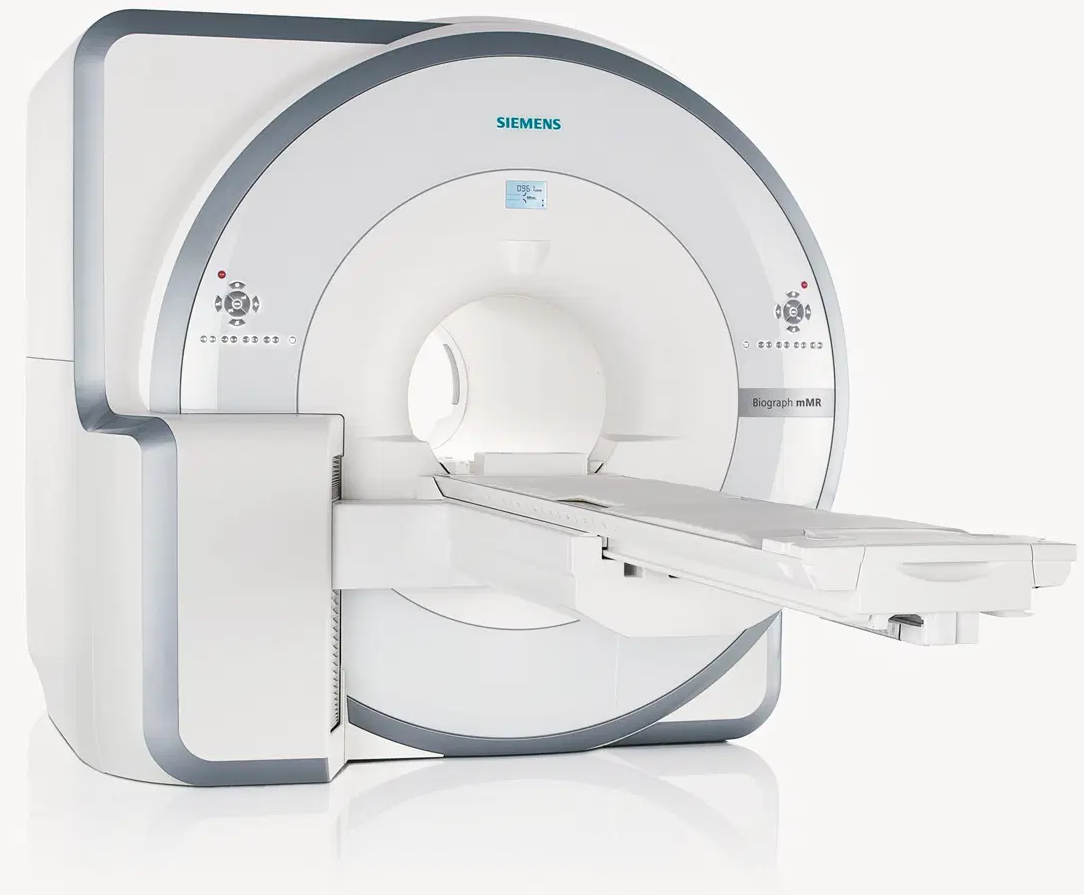
\includegraphics[height=2cm]{pet_machine2.png}};
			\node[anchor=north west,right=1cm of C2,yshift=-1cm] (ttac_image) {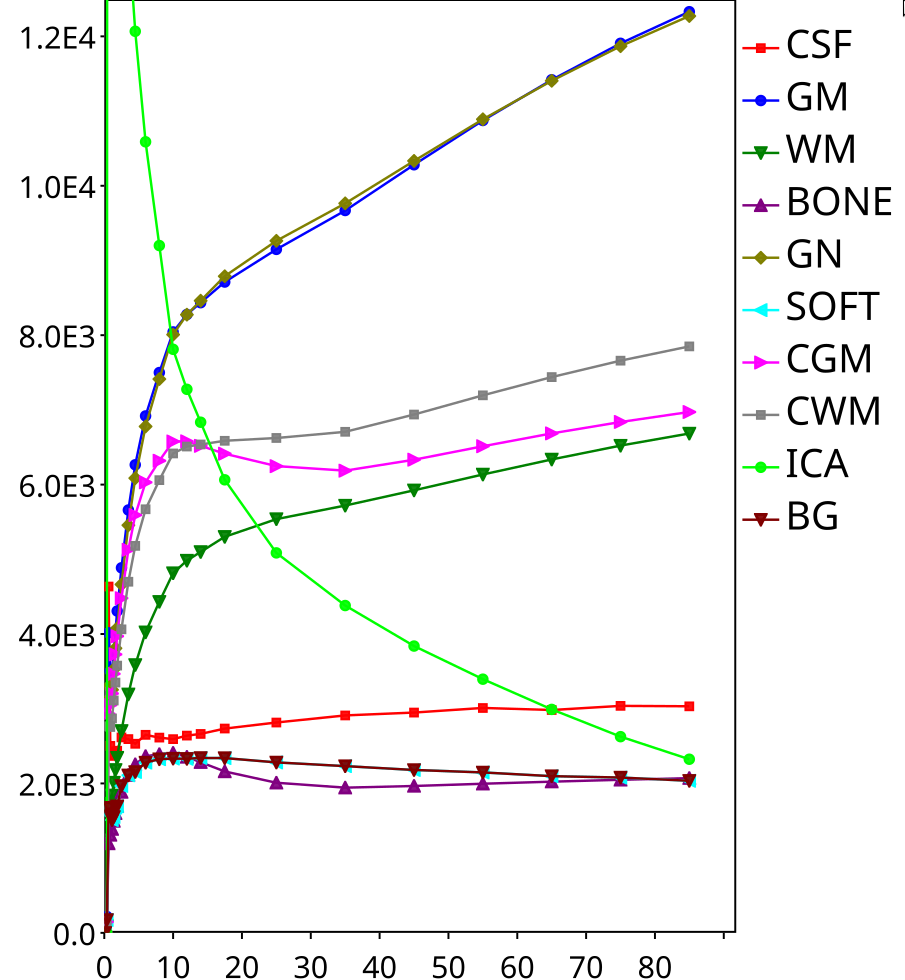
\includegraphics[width=4cm]{ttacs.png}};
			\node[above=0cm of ttac_image]{\small{Time Activity Curve (TAC)}};
		\end{scope}
	\end{tikzpicture}
\end{frame}

\begin{frame}{Input Function}
	\centering
	\begin{itemize}
		\item \textbf{Arterial Input Function (AIF)}: Continuous arterial sampling using a catheter
		      \begin{itemize}
			      \item The \textit{gold} standard
			      \item Invasive and uncomfortable
			      \item Labour intensive and error prone
		      \end{itemize}
		\item \textbf{Population-Based Input Function (PBIF):} Average blood activity based on set of subjects
		\item \textbf{Image-Derived Input Function (IDIF):}
		      Direct extraction of blood radioactivity from the PET image
	\end{itemize}

	\begin{center}
		\begin{minipage}{0.34\textwidth}
			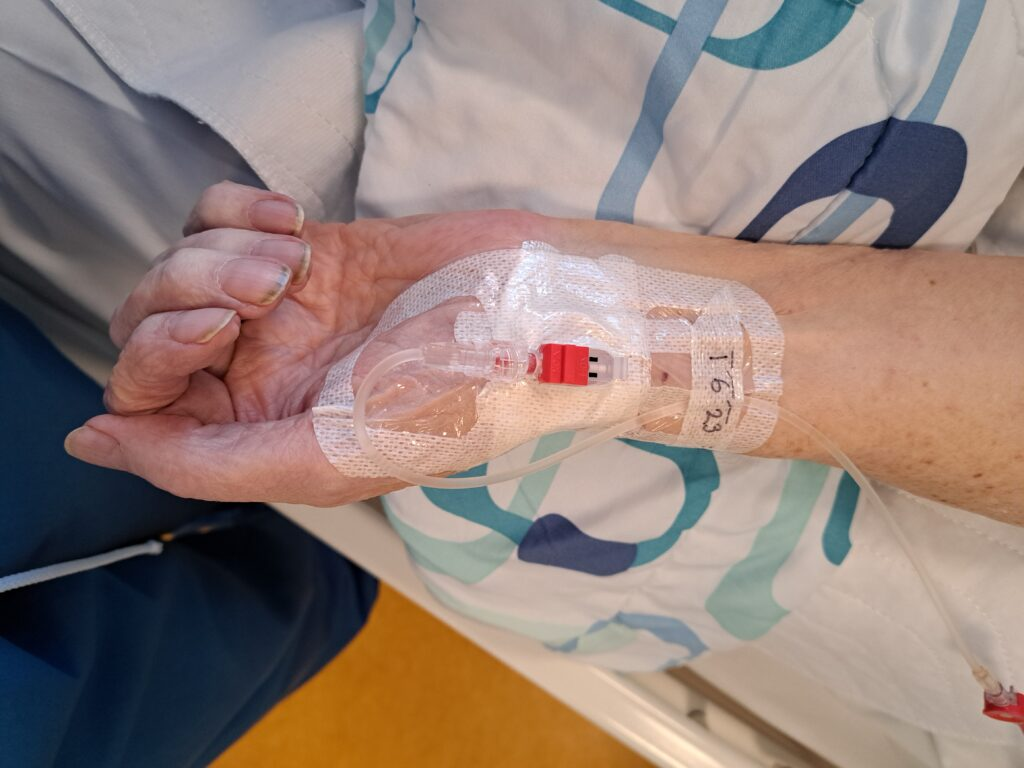
\includegraphics[width=\linewidth]{catheter2.jpg}
		\end{minipage}
		\begin{minipage}{0.36\textwidth}
			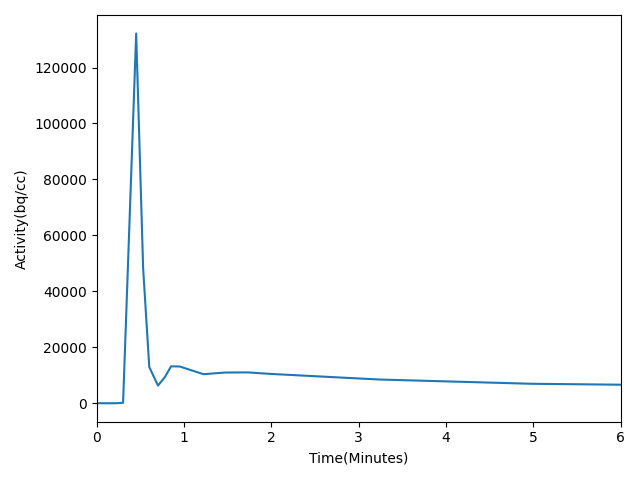
\includegraphics[width=\linewidth]{aif.png}
		\end{minipage}
		\vfill
	\end{center}

\end{frame}

\begin{frame}{How to do IDIF?}
	% \begin{enumerate}
	% 	\item Locate a major artery
	%        \item 
	% \end{enumerate}

	% ines: add a curve for IDIF 
	\begin{tikzpicture}[
			node distance=1cm,
			auto,
			>=Stealth,
			mybox/.style={draw, rounded corners, rectangle, minimum width=3cm, minimum height=1cm, align=center}
		]
		\node[mybox, visible on=<1->] (locate){Locate an Artery};
		\node[mybox, below=of locate, visible on=<1->] (mask) {Obtain an Accurate Mask};
		\node[mybox, below=of mask, visible on=<1->] (apply) {Apply to Dynamic PET};
		\node[mybox, below=of apply, sharp corners, visible on=<1->] (idif) {IDIF};

		\node[left=of mask]{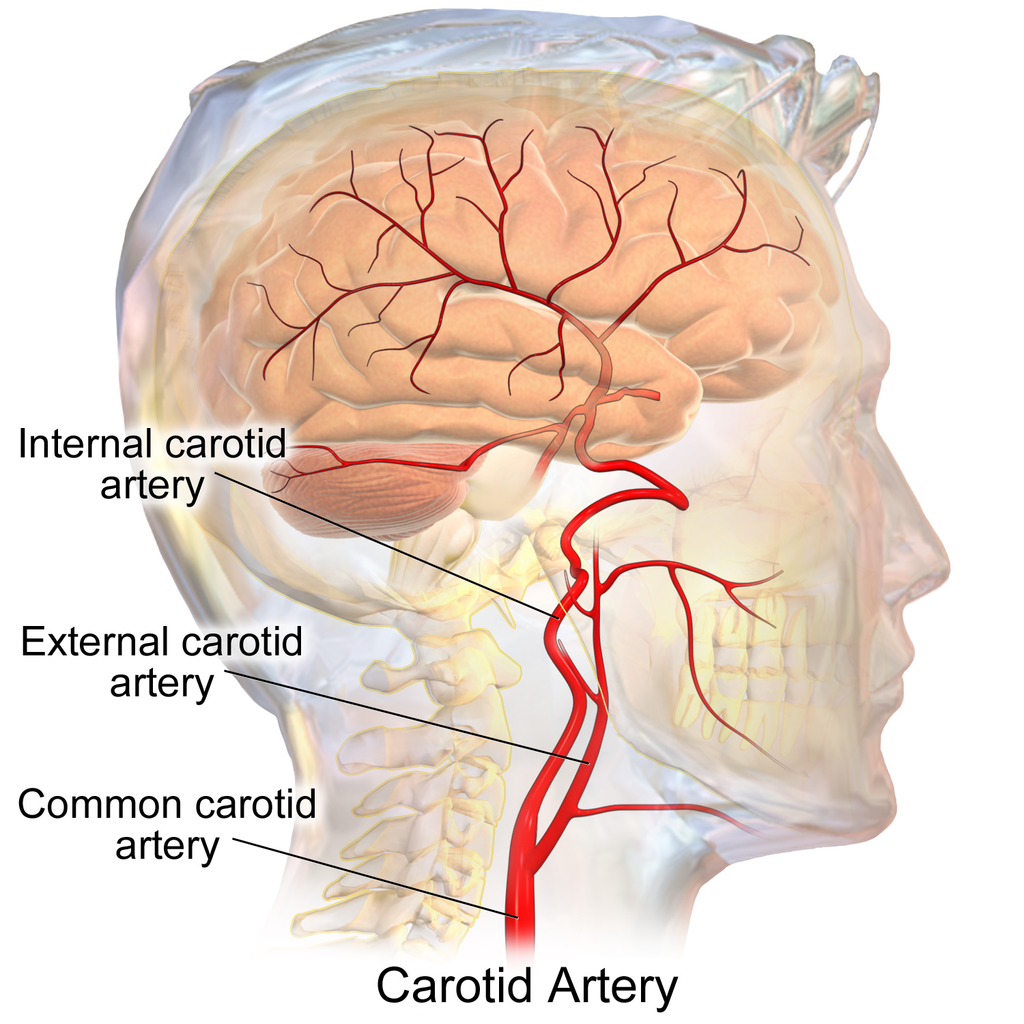
\includegraphics[width=4cm]{carotid_structure.png}};
		\node[right=of mask,visible on =<2->](pet){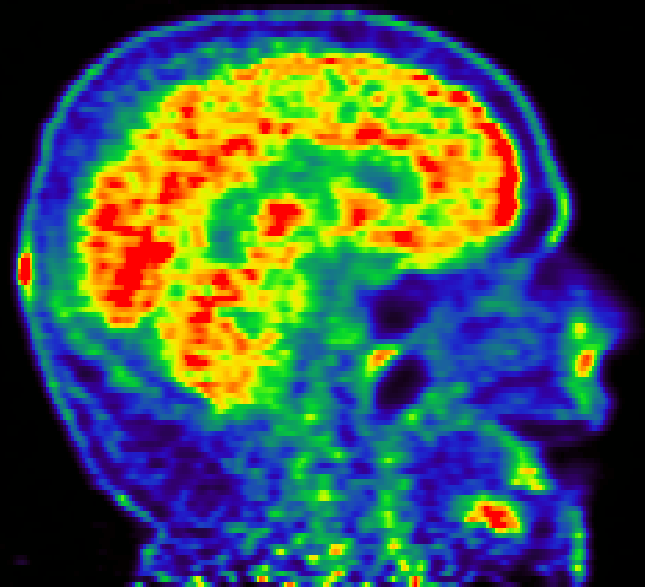
\includegraphics[width=4cm]{pet_slice_example.png}};
		\node[below=0cm of pet, visible on =<3->](idif2){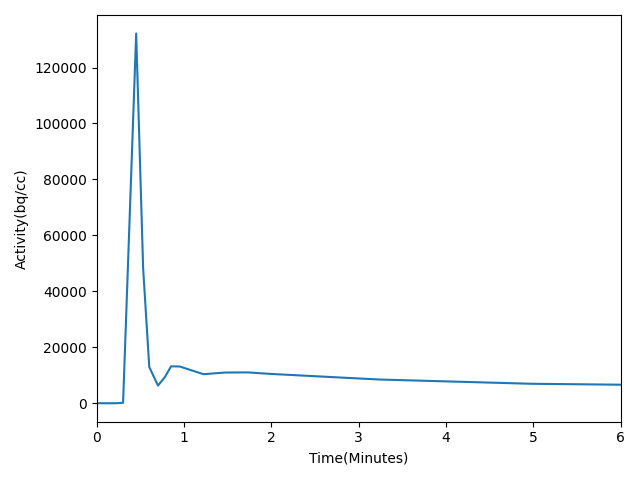
\includegraphics[width=4cm]{aif.png}};
		% \node[above=0cm of pet]{PET};

		\draw[->] (locate) -- (mask);
		\draw[->] (mask) -- (apply);
		\draw[->] (apply) -- (idif);
	\end{tikzpicture}
\end{frame}


\begin{frame}{Artery Segmentation Methods}
	\begin{columns}
		\small
		\begin{column}{0.7\textwidth}
			\textbf{PET Only:}
			\begin{itemize}
				\item \textbf{\citeauthoryear{young2023image}}: Manual delineation from early PET frames
				\item \textbf{\citeauthoryear{vestergaard2021validation}}: Semi-automatic thresholding
				\item \textbf{\citeauthoryear{chavan2024end}}: Fully Automatic U-NET Network
			\end{itemize}
			\vspace{2em}
			\uncover<3->{
				\textbf{Multi-Modal:}
				\begin{itemize}
					\item \textbf{\citeauthoryear{sundar2019towards}}: Seeded region growing on TOF-MRA (semi-automatic)
					\item \textbf{\citeauthoryear{sari2017estimation}}: Fully automatic using TOF-MRA
					\item \textbf{\citeauthoryear{rahman2024deep}}: Deep learning on T1w MRI
				\end{itemize}%
			}
		\end{column}

		\begin{column}{0.3\textwidth}
			\begin{tikzpicture}[
					node distance=1cm,
					auto,
					>=Stealth,
					mybox/.style={draw, rounded corners, rectangle, minimum width=3cm, minimum height=1cm, align=center}
				]

				\node[visible on=<1>](pet){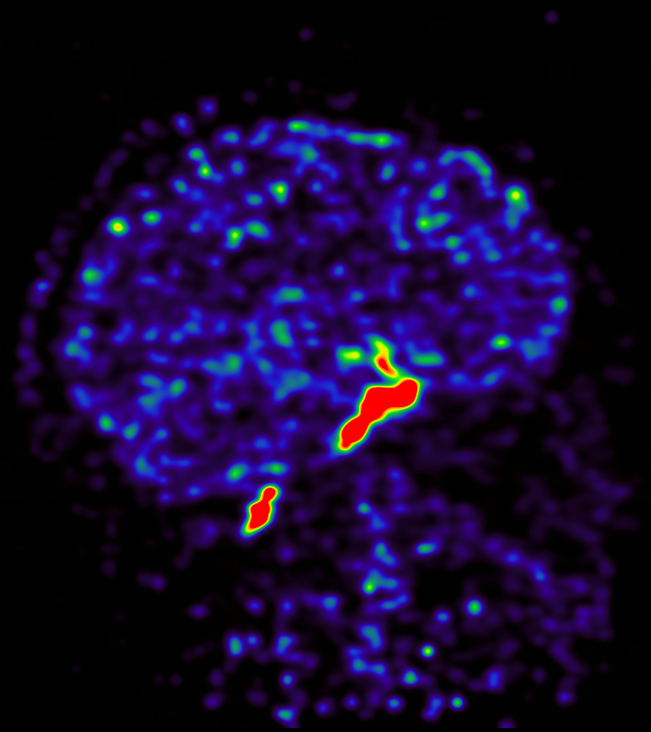
\includegraphics[height=4cm]{cpet.png}};
				\node[visible on=<2->]{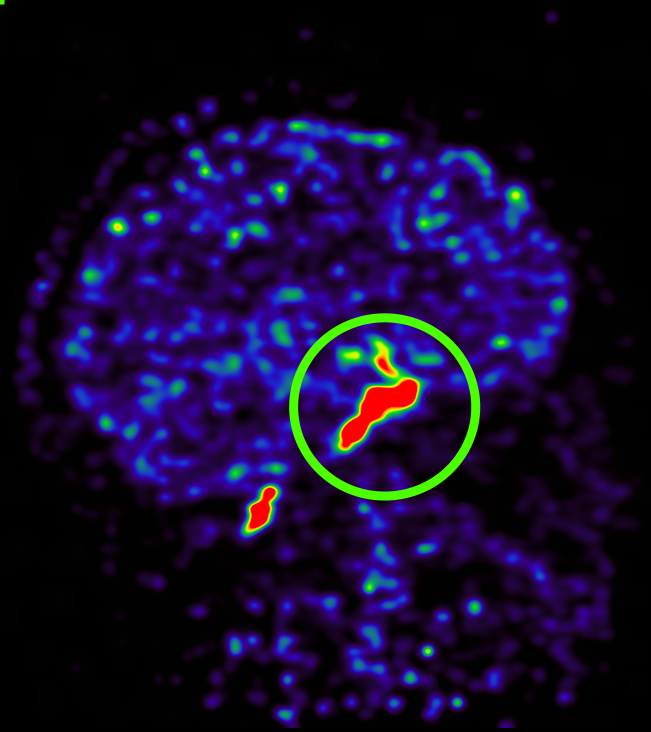
\includegraphics[height=4cm]{cpet2.png}};

				\node[below=2mm of pet, visible on=<3>](tof){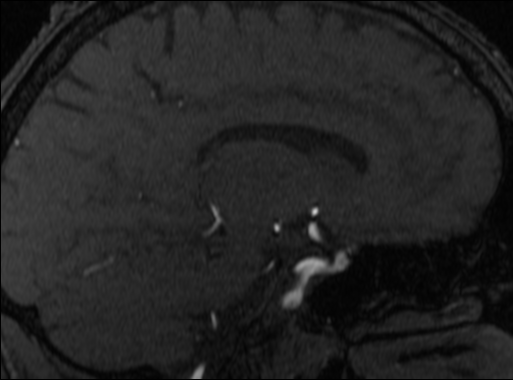
\includegraphics[height=3cm]{ctof.png}};
				\node[below=2mm of pet, visible on=<3->]{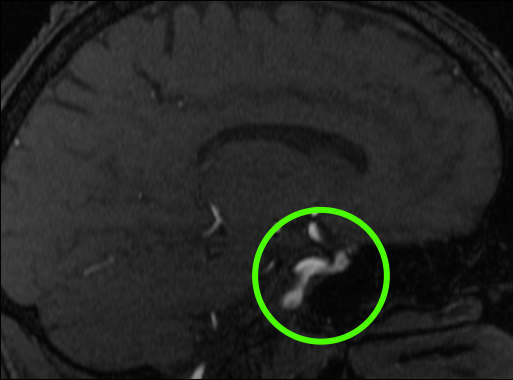
\includegraphics[height=3cm]{ctof2.png}};


				\def\tofshift{(10pt, 0pt)}
				\def\petshift{(12pt,-23pt)}

				\draw[->,bend right=15,very thick,green,visible on=<3->]
				([shift=\tofshift]tof.center) to ([shift=\petshift]pet.center);
			\end{tikzpicture}
		\end{column}
	\end{columns}
\end{frame}

\begin{frame}{Objective}
	% \centering\Large{Develop a model for Internal Carotid Artery segmentation from TOF-MR Angiography for Image-Derived Input Function}
	\centering\Large{To replace the Invasive AIF:\\Obtain an accurate \textbf{segmentation} of the \textbf{carotids} from \textbf{MR-Angiography} for Image-Derived Input Function}
	% Develop a model for Internal Carotid Artery segmentation from TOF-MR Angiography for Image-Derived Input Function}
\end{frame}

\section{Methods}

\begin{frame}{Internal Carotid Artery(ICA) Segmentation Pipeline}
	\centering
	\begin{tikzpicture}[
			node distance=1.5cm,
			auto,
			>=Stealth,
			mybox/.style={draw, rounded corners, rectangle, minimum width=3cm, minimum height=1cm, align=center}
		]

		\node[mybox, alt=<2>{draw=red,very thick} ] (input) {TOF-MRA};

		\node[mybox, alt=<4>{draw=red,very thick}, visible on=<4->, right=of input, fill=yellow!20] (cuboid) { Cuboid Mask\\Application};

		\node[mybox, alt=<{3,5}>{draw=red,very thick}, right=of cuboid] (thresh) {High Intensity\\ Thresholding};
		% \node[       alt=<{3,5}>{draw=red,very thick}, above=1mm of thresh.north] (hist) {\includegraphics[width=2cm]{hist.png}};

		% \node[mybox, alt=<5>{draw=red,very thick}, right=of cuboid] (thresh2) {Adaptive Histogram\\ Thresholding};
		% \node[       alt=<5>{draw=red,very thick}, above=1mm of thresh.north] (hist2) {\includegraphics[width=2cm]{hist.png}};

		\node[mybox, alt=<5>{draw=red,very thick}, below=of thresh] (growing) {Largest 2 Volumes};
		\node[mybox, alt=<6>{draw=red,very thick}, below=of growing,fill=green] (mask) {Carotid\\Mask};
		\node[mybox, alt=<7>{draw=red,very thick}, left=of growing] (dilation) {Dilation};
		\node[mybox, alt=<7>{draw=red,very thick}, below=of dilation,fill=blue!80] (bg_mask) {Background Mask\\(surrounding tissue)};

		\node[align=center,below=1cm of input.south,visible on=<1-2>] (image) {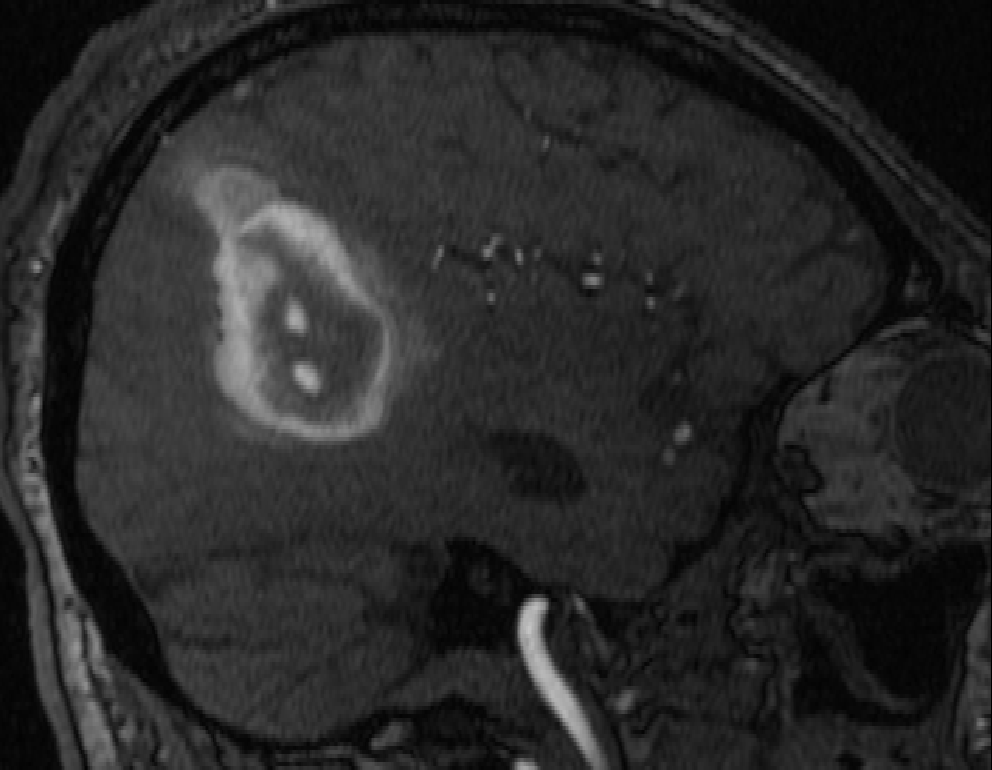
\includegraphics[width=4.5cm]{segmentation_raw.png}};
		\node[align=center,below=1cm of input.south,visible on=<3>] (image) {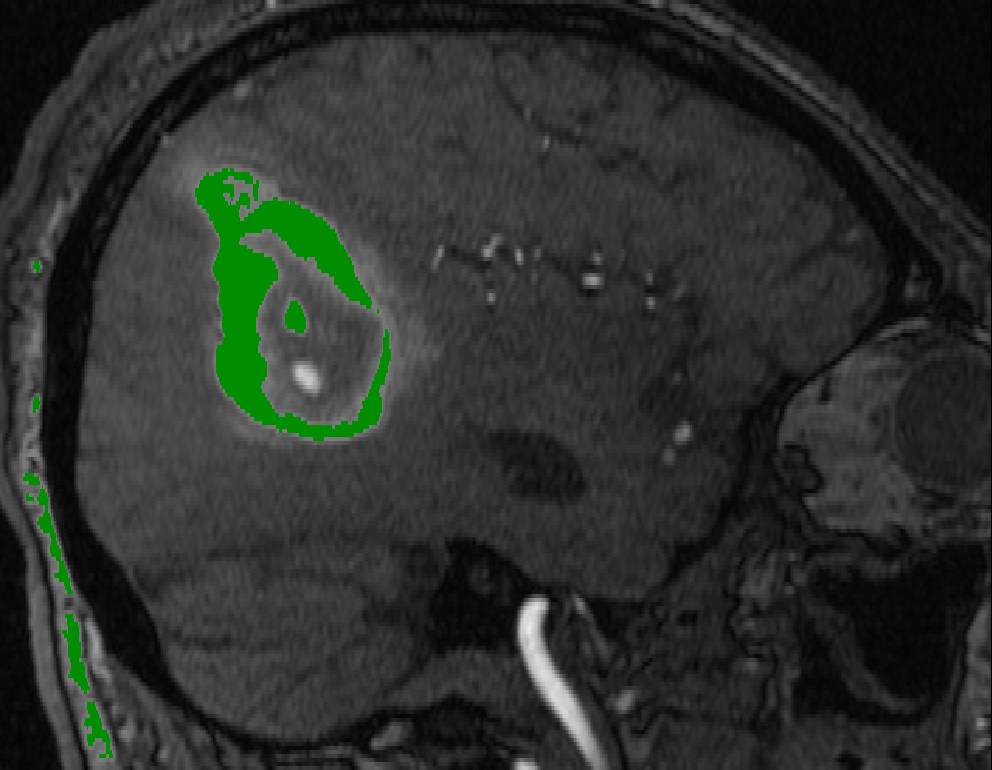
\includegraphics[width=4.5cm]{segmentation_no_bbox.png}};
		\node[align=center,below=1cm of input.south,visible on=<4>] (image) {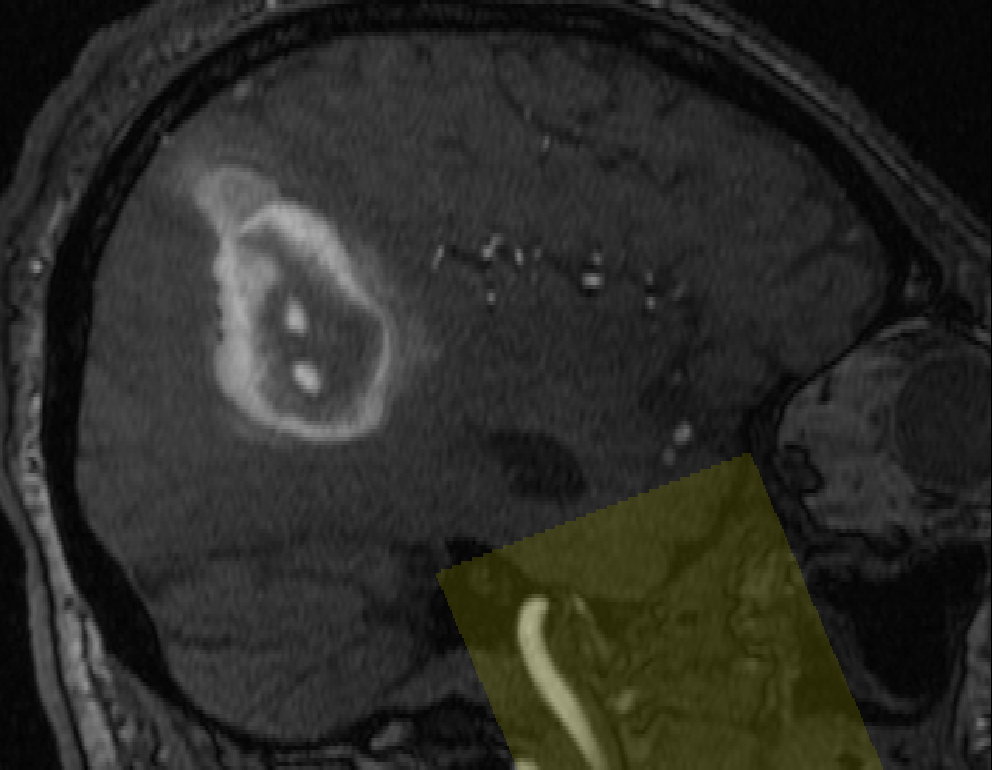
\includegraphics[width=4.5cm]{segmentation_just_bbox.png}};
		\node[align=center,below=1cm of input.south,visible on=<5-6>] (image) {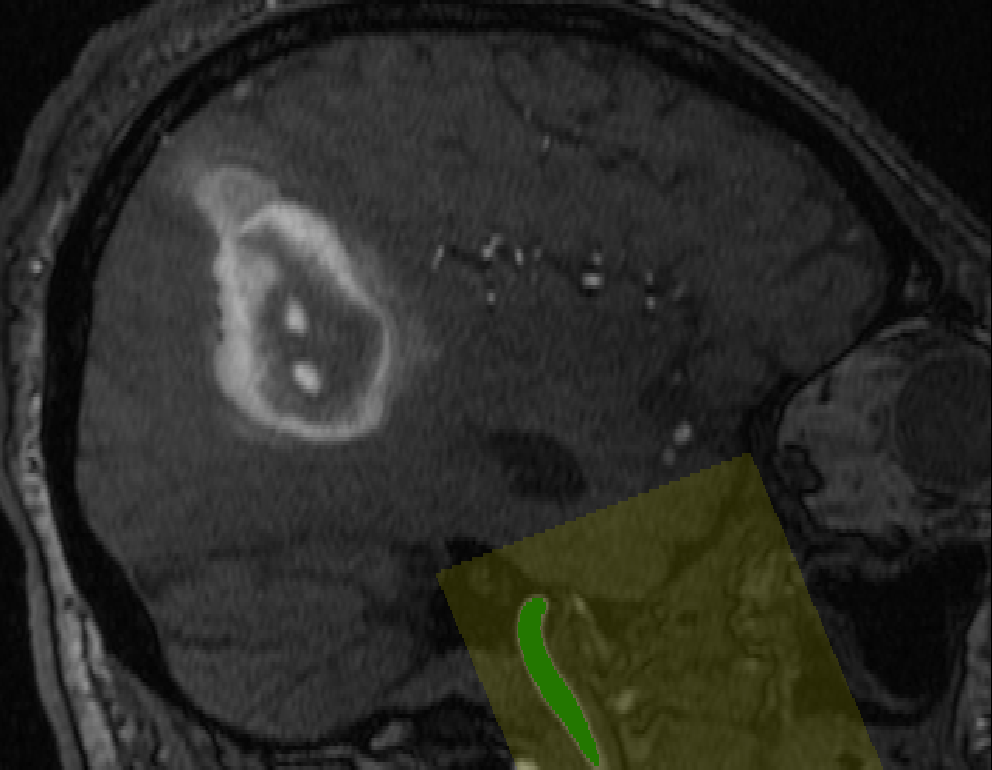
\includegraphics[width=4.5cm]{segmentation_with_bbox.png}};
		\node[align=center,below=1cm of input.south,visible on=<7->] (image) {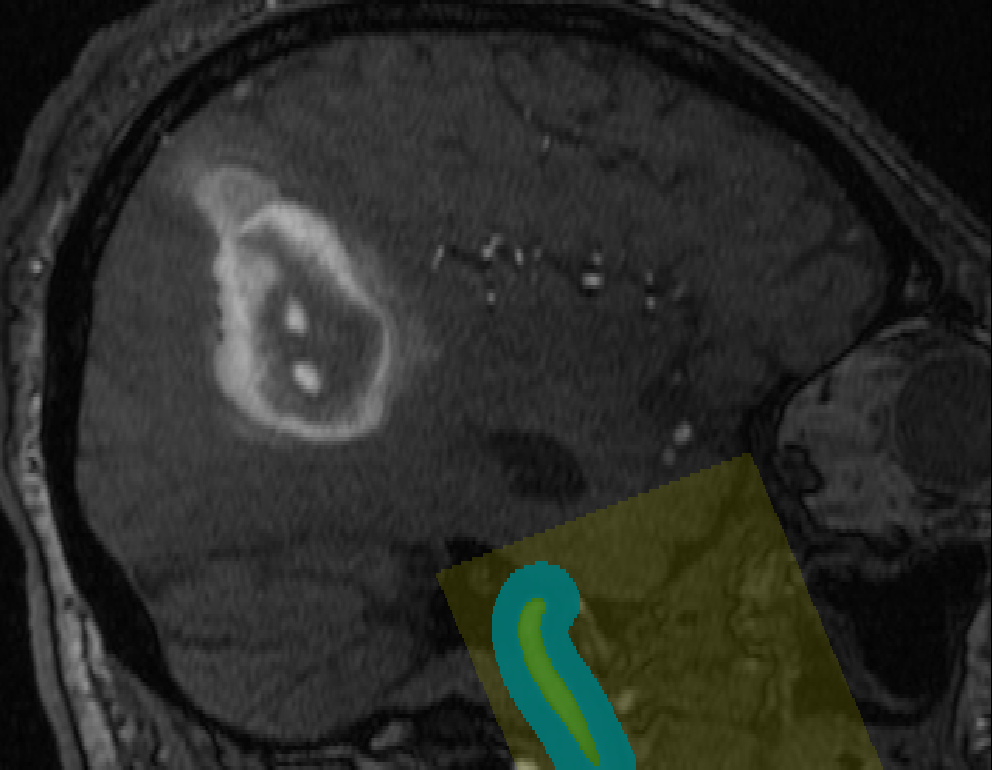
\includegraphics[width=4.5cm]{segmentation_with_bbox_and_bg.png}};


		\draw[->,visible on=<4->] (input) -- (cuboid);
		\draw[->,visible on=<4->] (cuboid) -- (thresh);
		\draw[->,visible on=<-3>] (input) -- (thresh);

		\draw[->] (thresh) -- (growing);
		\draw[->] (growing) -- (mask);
		\draw[->] (growing) -- (dilation);
		\draw[->] (dilation) -- (bg_mask);

	\end{tikzpicture}
\end{frame}

% \begin{frame}[t]{IDIF Challenges:}
% 	\textbf{1) Segmentation:} A vessel must be accurately segmented to extract the input function from the PET
% 	\vfill
% 	\textbf{2) Partial Volume Effect:} Signals mix with surrounding tissues (Spill-in \& Spill-out).
%
% 	\begin{center}
% 		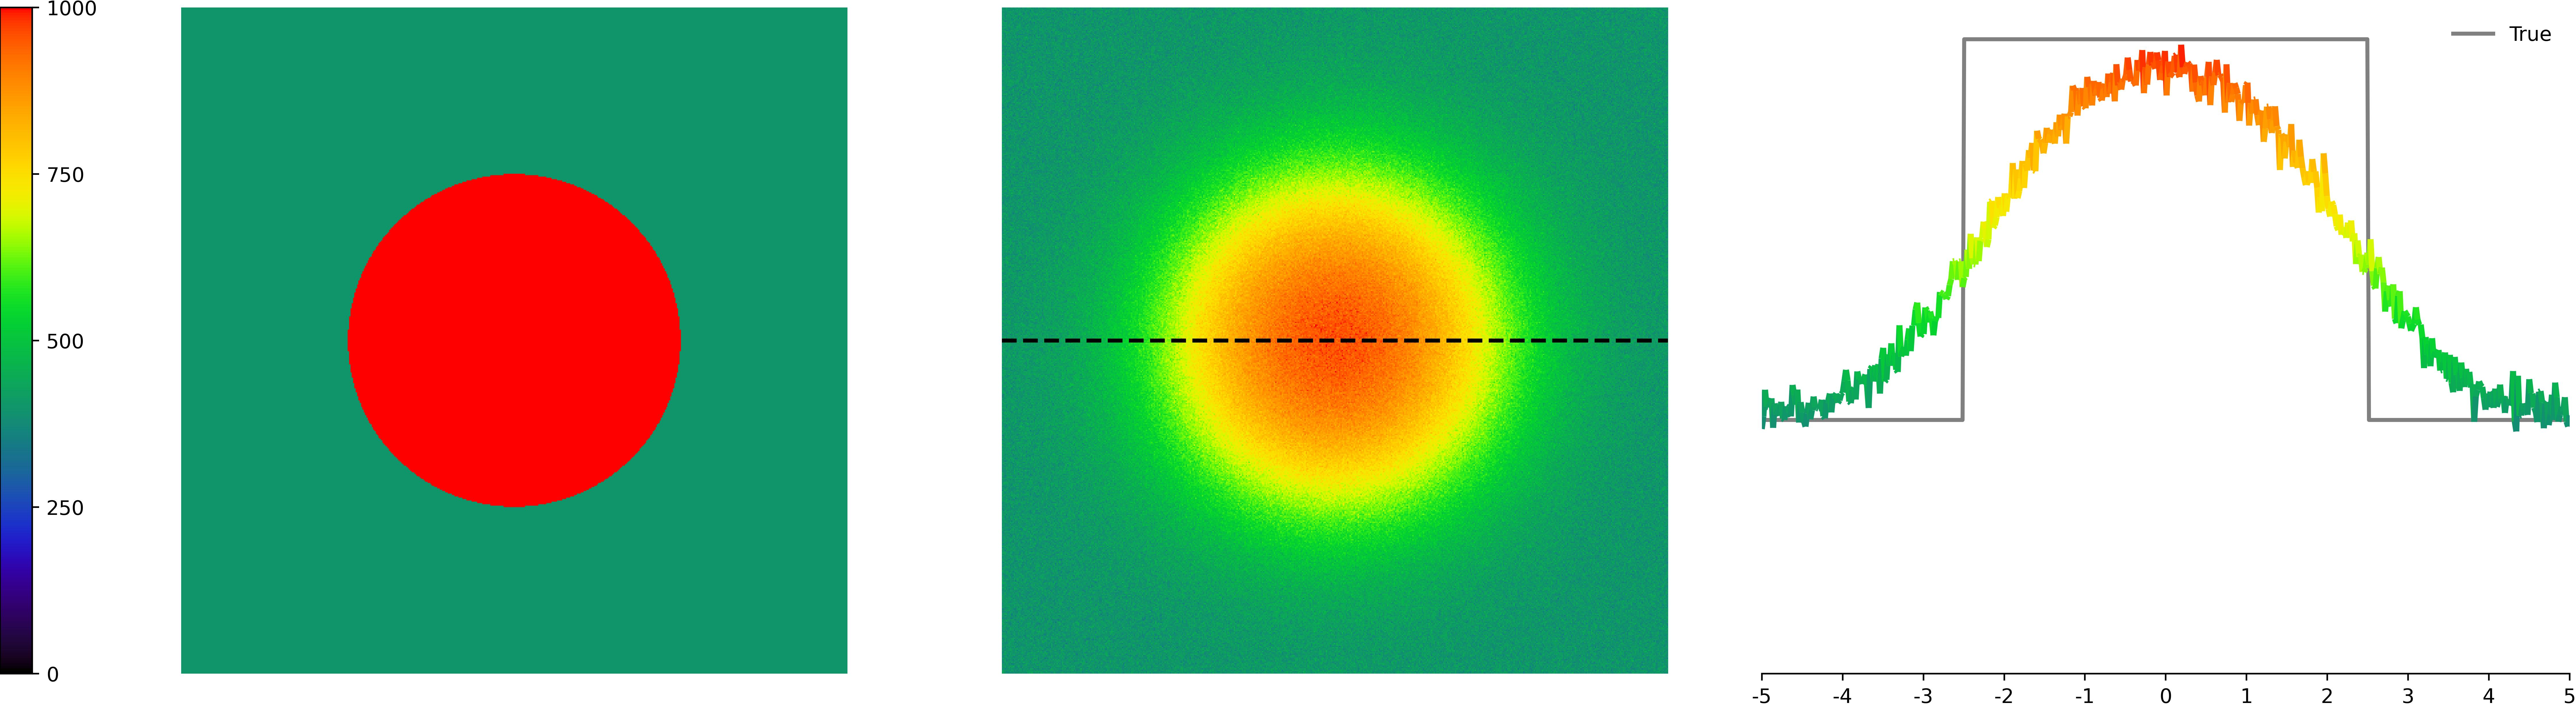
\includegraphics[width=0.9\textwidth]{pve.jpg}
% 	\end{center}
% \end{frame}

\begin{frame}{Image Derived Input Function (IDIF)}
	\resizebox{0.95\textwidth}{!}{%
		\begin{tikzpicture}[
				node distance=1cm,
				auto,
				>=Stealth,
				mybox/.style={draw, rounded corners, rectangle, minimum width=3cm, minimum height=1cm, align=center}
			]
			\node[mybox] (mri) {MR Angiography};
			\node[mybox,right=of mri] (artery) {Artery Mask};
			\node[mybox,below=of artery] (pet) {Dynamic PET};
			% \coordinate (mid) at ($(artery)!0.5!(pet)$);
			\node[mybox,right=3 of pet](idif){Image Derived\\Input Function};
			\node[above=0cm of mri,visible on=<1>]{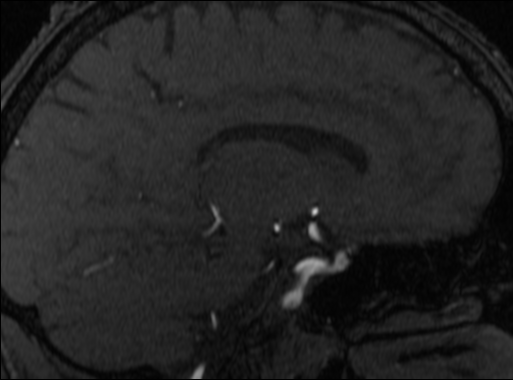
\includegraphics[height=2.5cm]{ctof.png}};
			\node[above=0cm of mri,visible on=<2->]{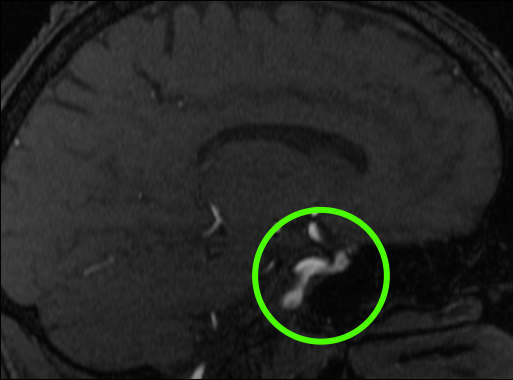
\includegraphics[height=2.5cm]{ctof2.png}};

			\node[below=0cm of mri,visible on=<1>]{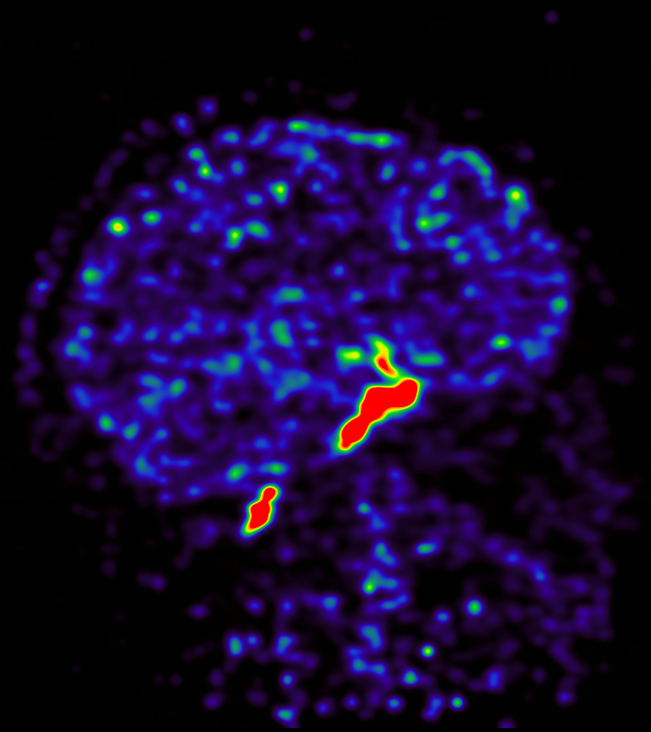
\includegraphics[height=2.5cm]{cpet.png}};
			\node[below=0cm of mri,visible on=<2->]{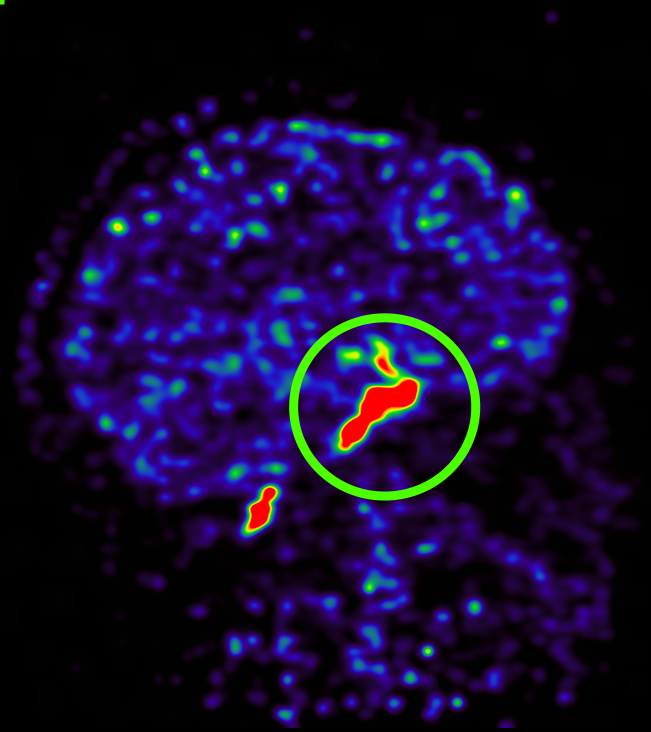
\includegraphics[height=2.5cm]{cpet2.png}};
			\node[above=0cm of artery,visible on=<2->]{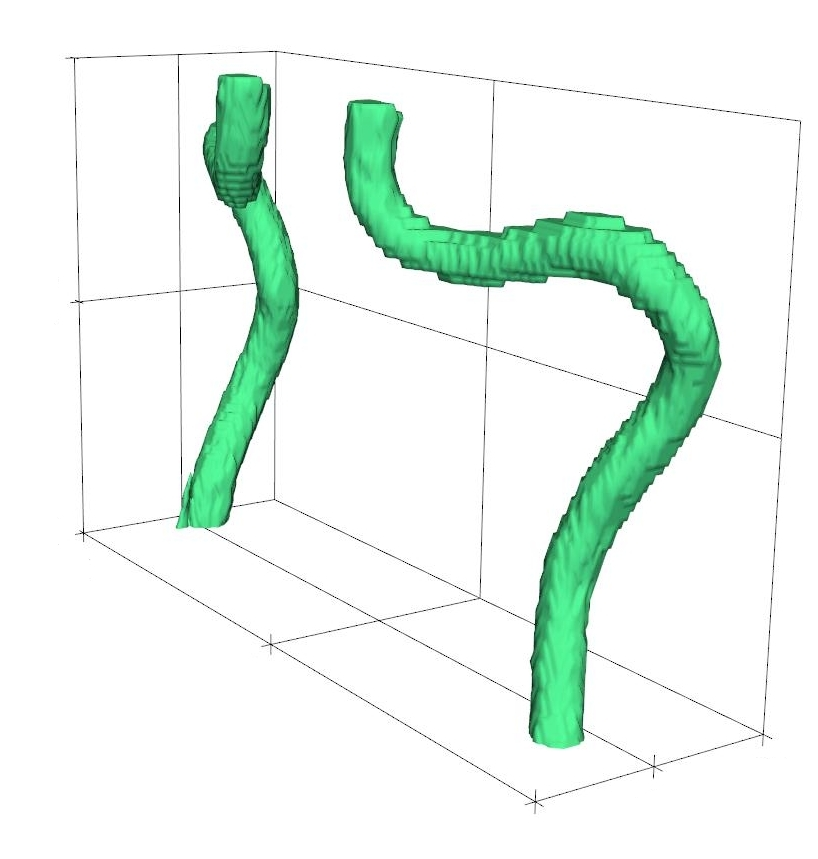
\includegraphics[height=2.5cm]{carotid_3d.jpg}};

			\node[anchor=south west,visible on=<3->] at($(pet.north east)+(1.2,0)$) {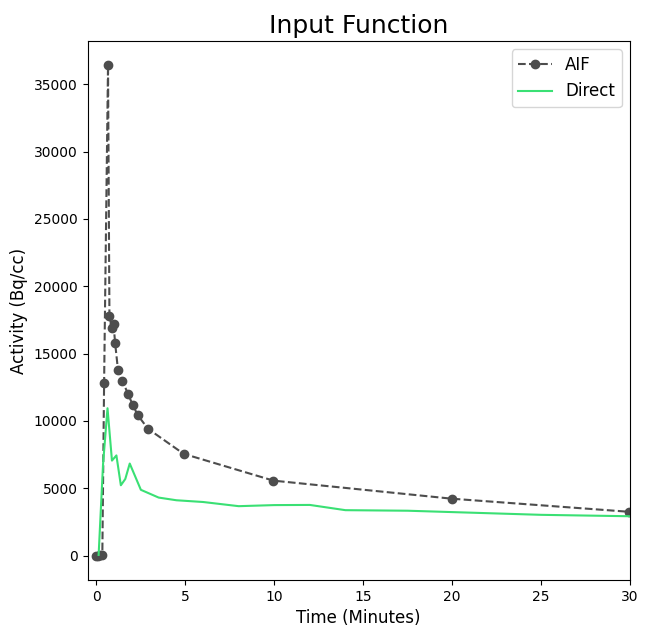
\includegraphics[width=6cm]{BADKA07504_1_infunc_direct2.png}};

			\draw[->] (mri.east) -- (artery.west);
			\draw[->] (artery.east) to[out=0, in=180] (idif.west);
			\draw[->] (pet.east) to[out=0, in=180] (idif.west);
		\end{tikzpicture}% 
	}
\end{frame}


\begin{frame}{Partial Volume Effect}
	\begin{center}
		\Large\textbf{Mixture of Activity with surrounding tissues\\(Spill-in \& Spill-out Effects)}

		% 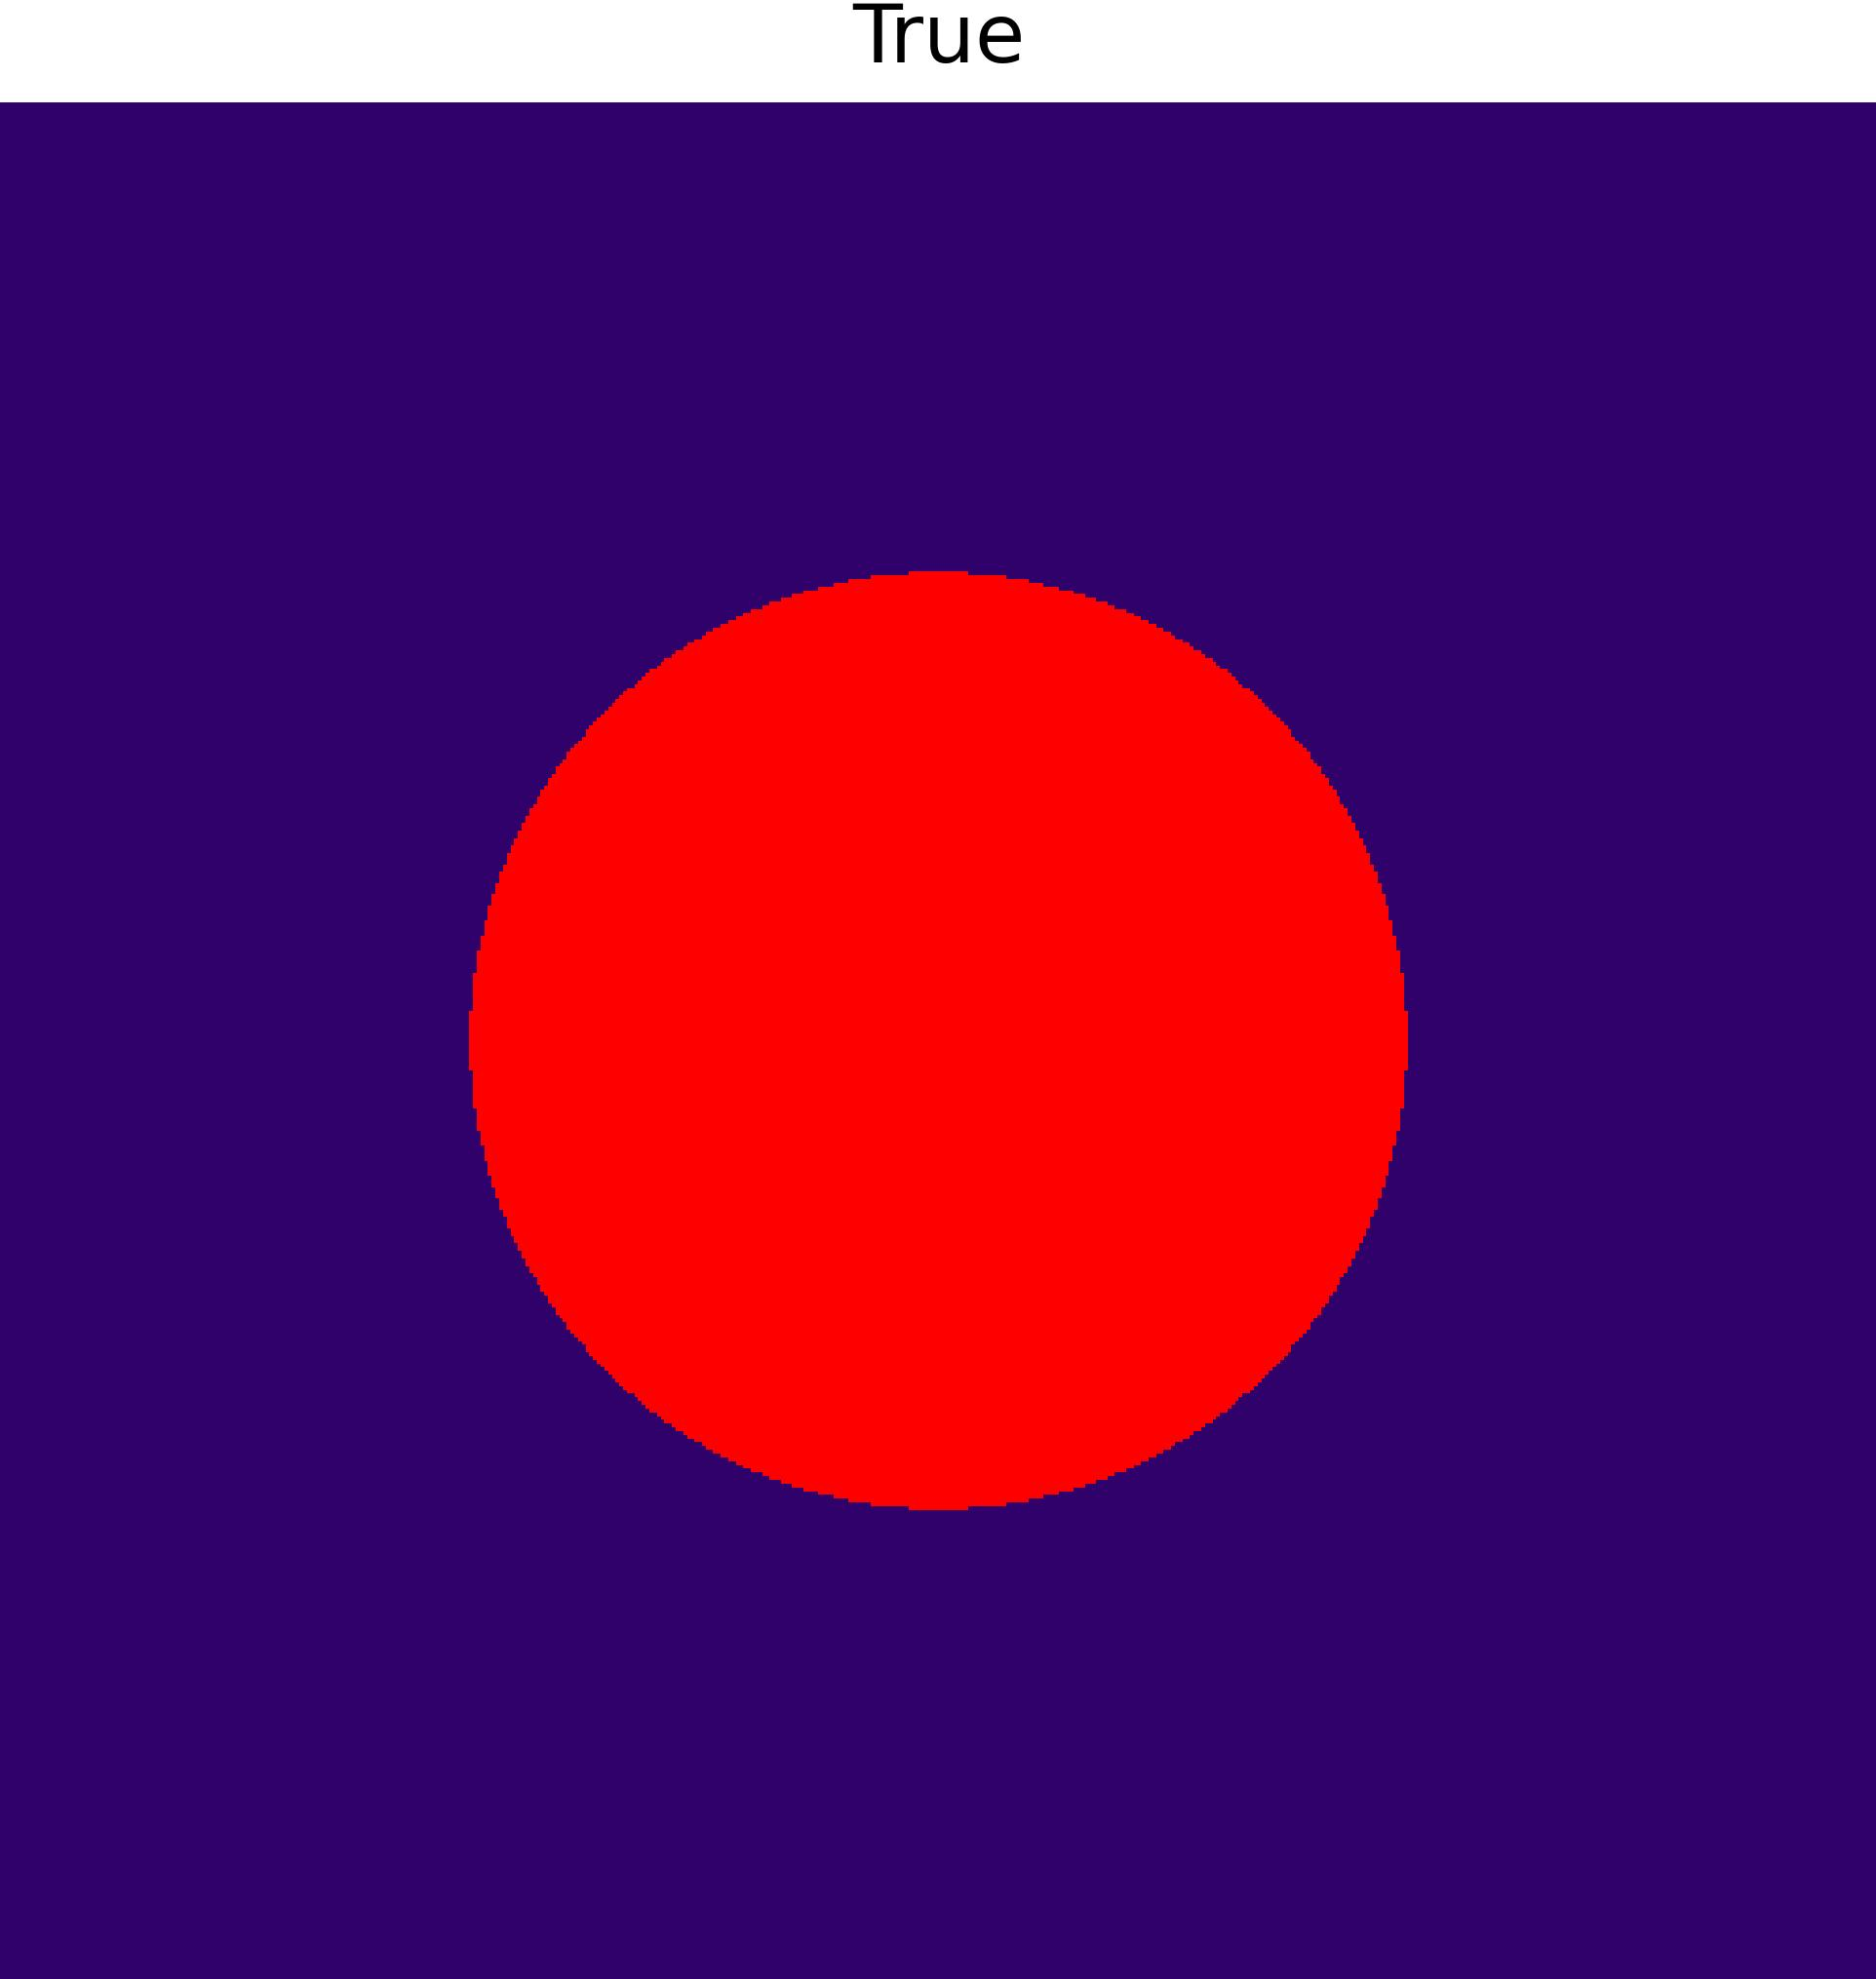
\includegraphics[height=5cm]{pve_true.jpg}
		\vfill
		\begin{tikzpicture}
			\node[anchor=north west, inner sep=0] (img)
			at (0,0) {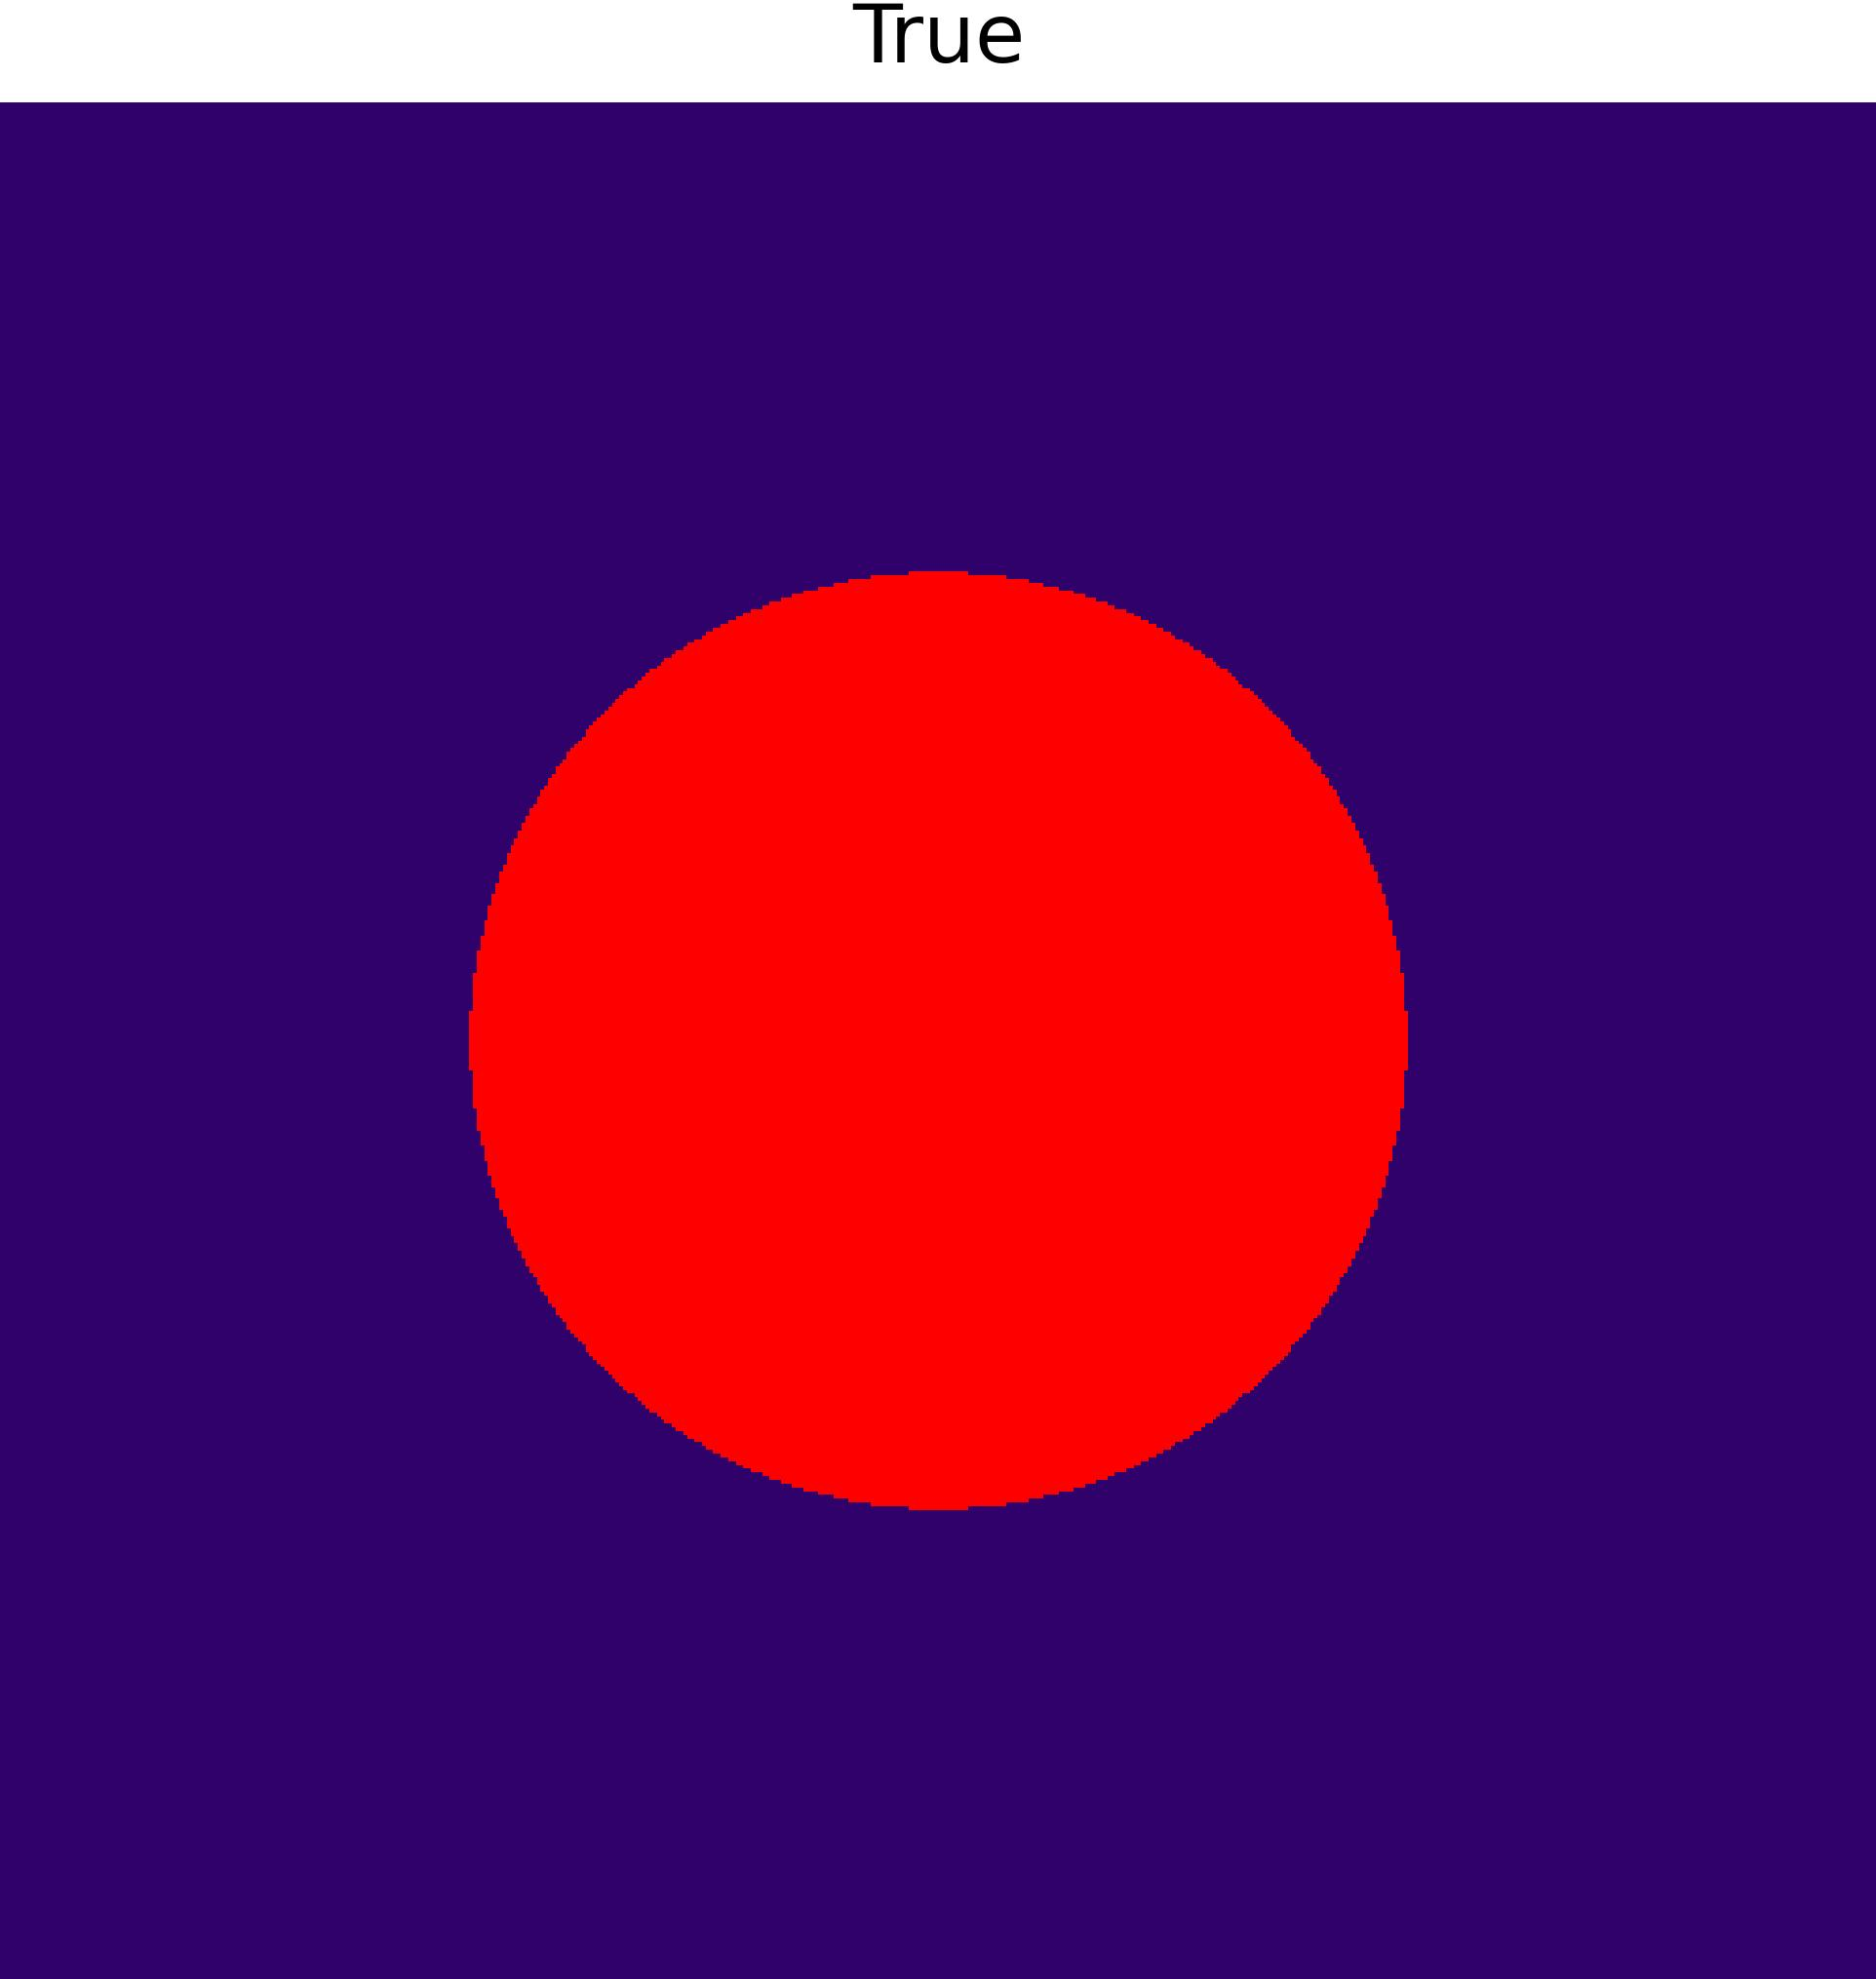
\includegraphics[height=5cm]{pve_true.jpg}};
			% \begin{scope}[x={(img.north east)}, y={(img.south west)},visible on=<2->]
			% 	\draw[->, >=stealth, bend left=30,thick, color=white]
			% 	(0.6,0.47) to node[above, text=white] {\small $\omega_{out}$} (0.85,0.47);
			% 	\draw[<-, >=stealth, bend right=30,thick, color=white]
			% 	(0.6,0.57) to node[below, text=white] {\small $\omega_{in}$} (0.85,0.57);
			% \end{scope}
		\end{tikzpicture}
		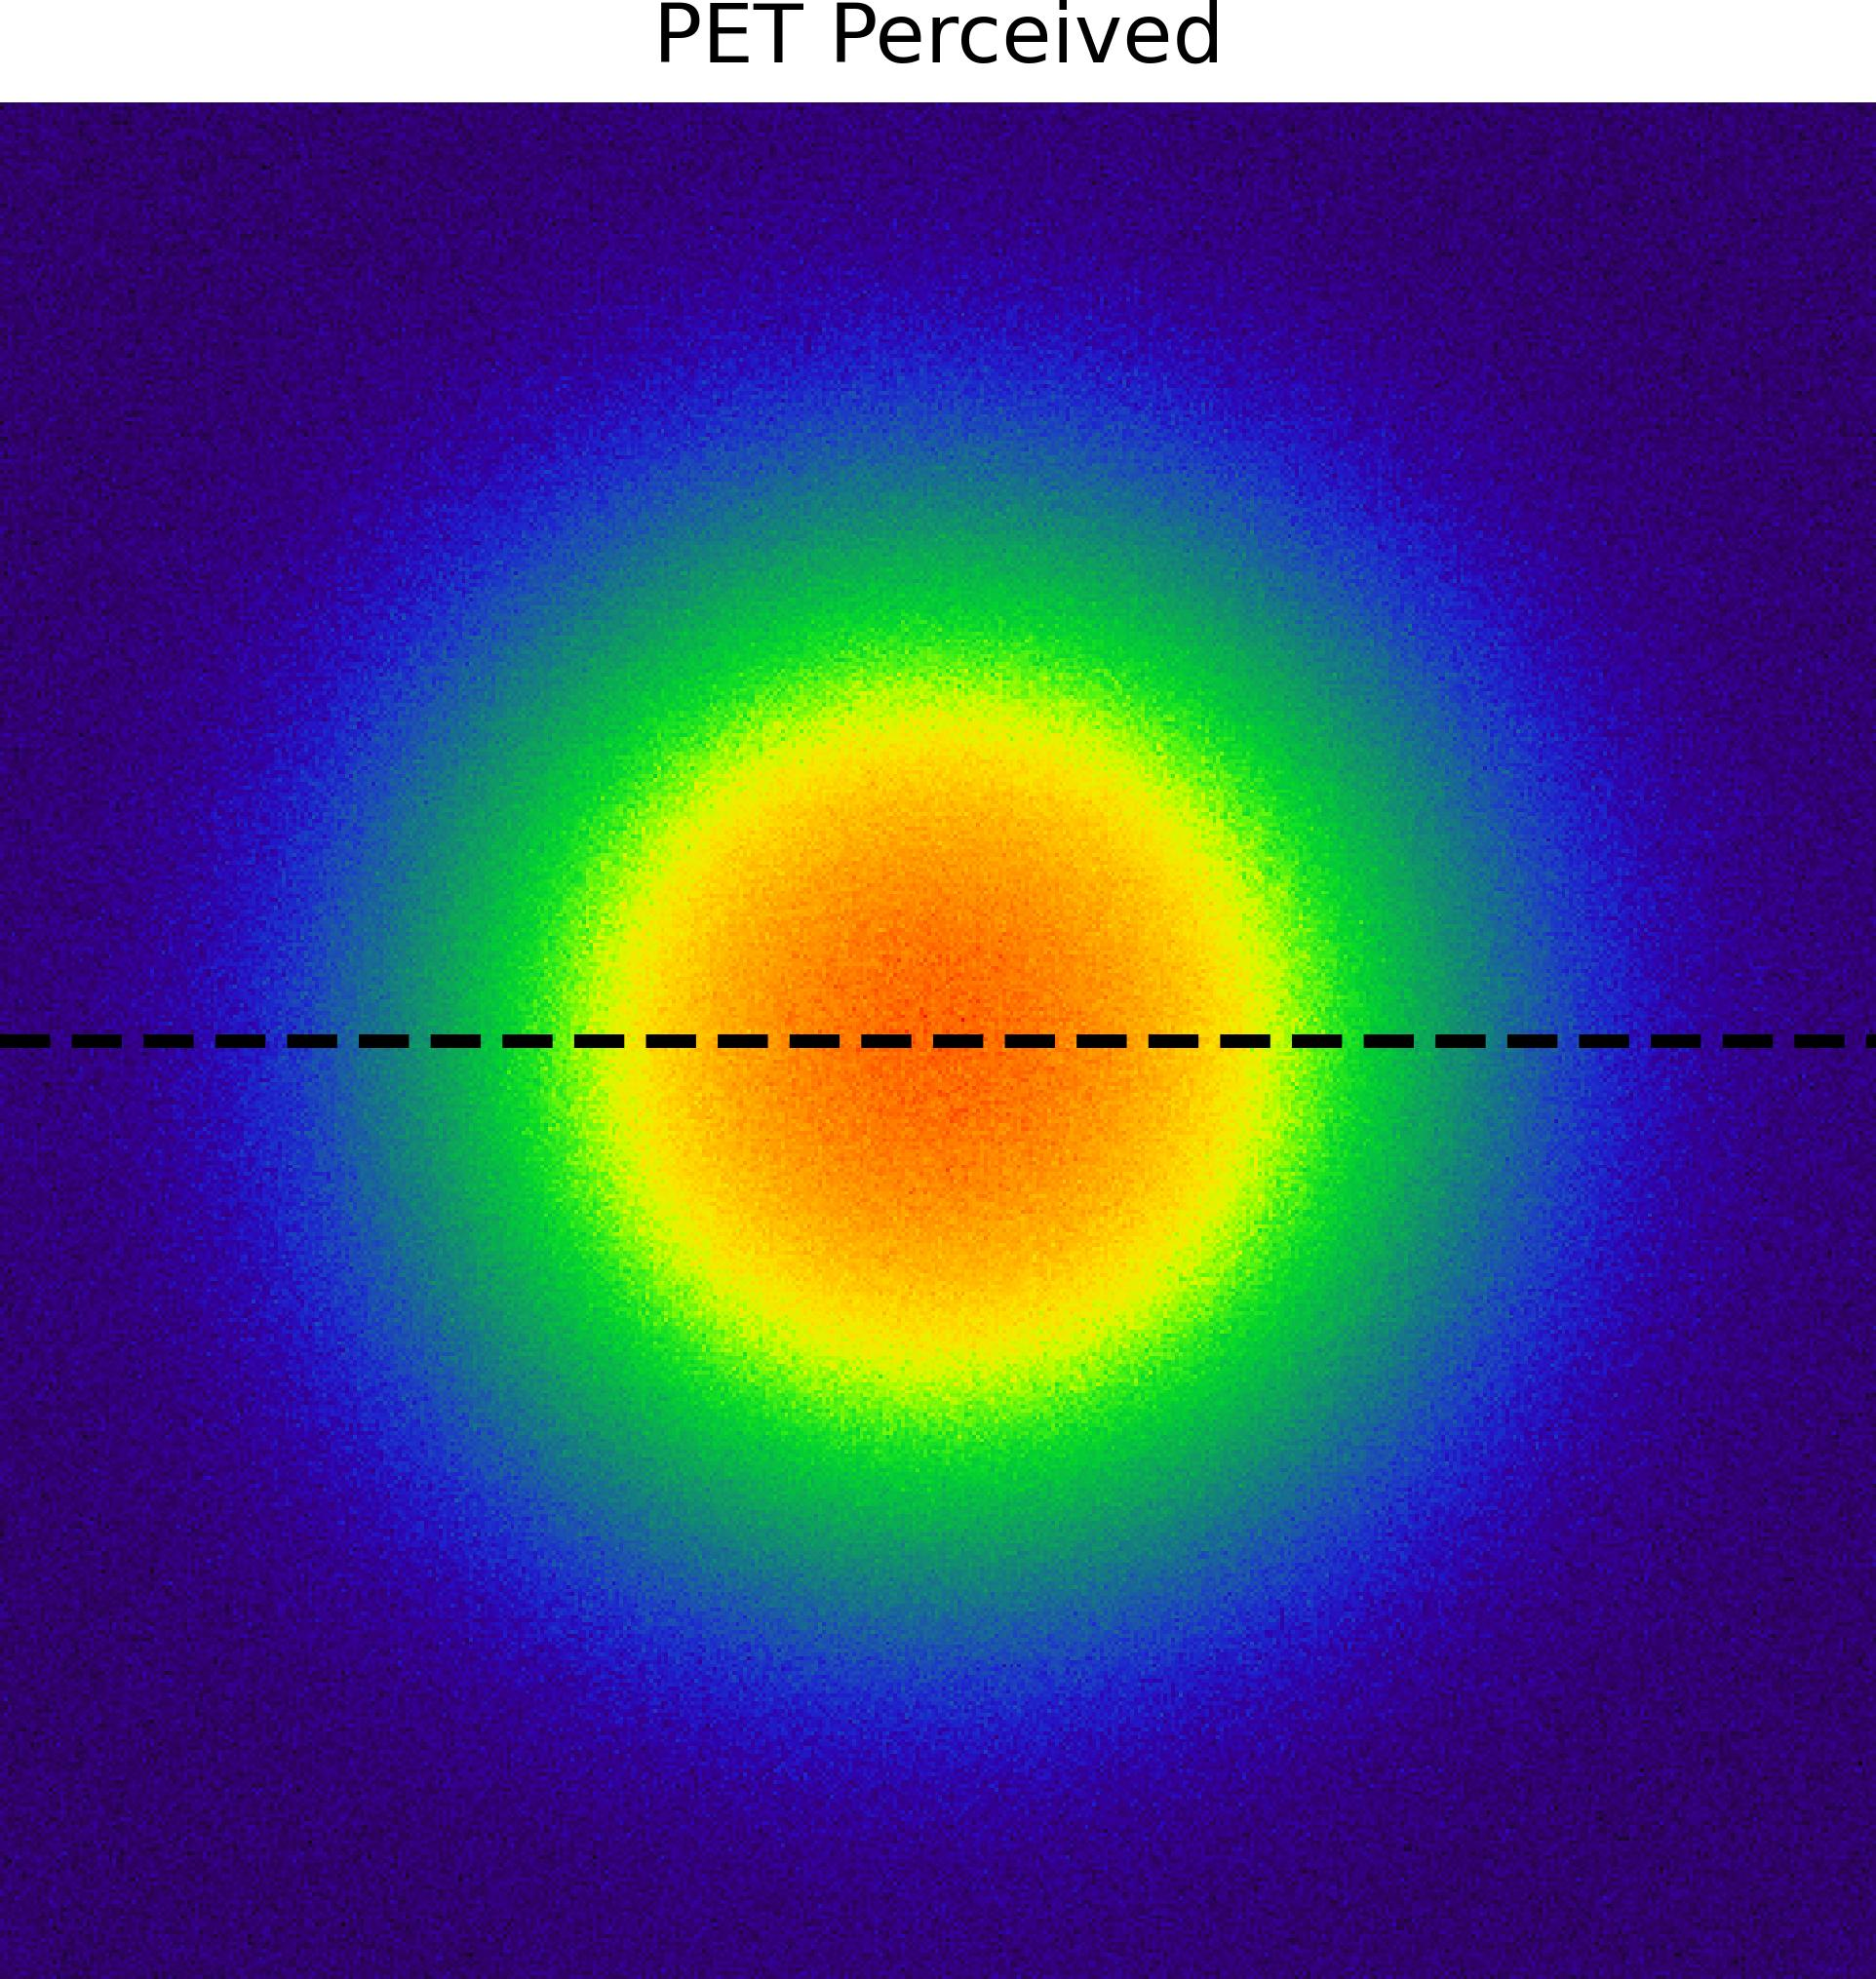
\includegraphics[height=5cm]{pve_perceived.jpg}
		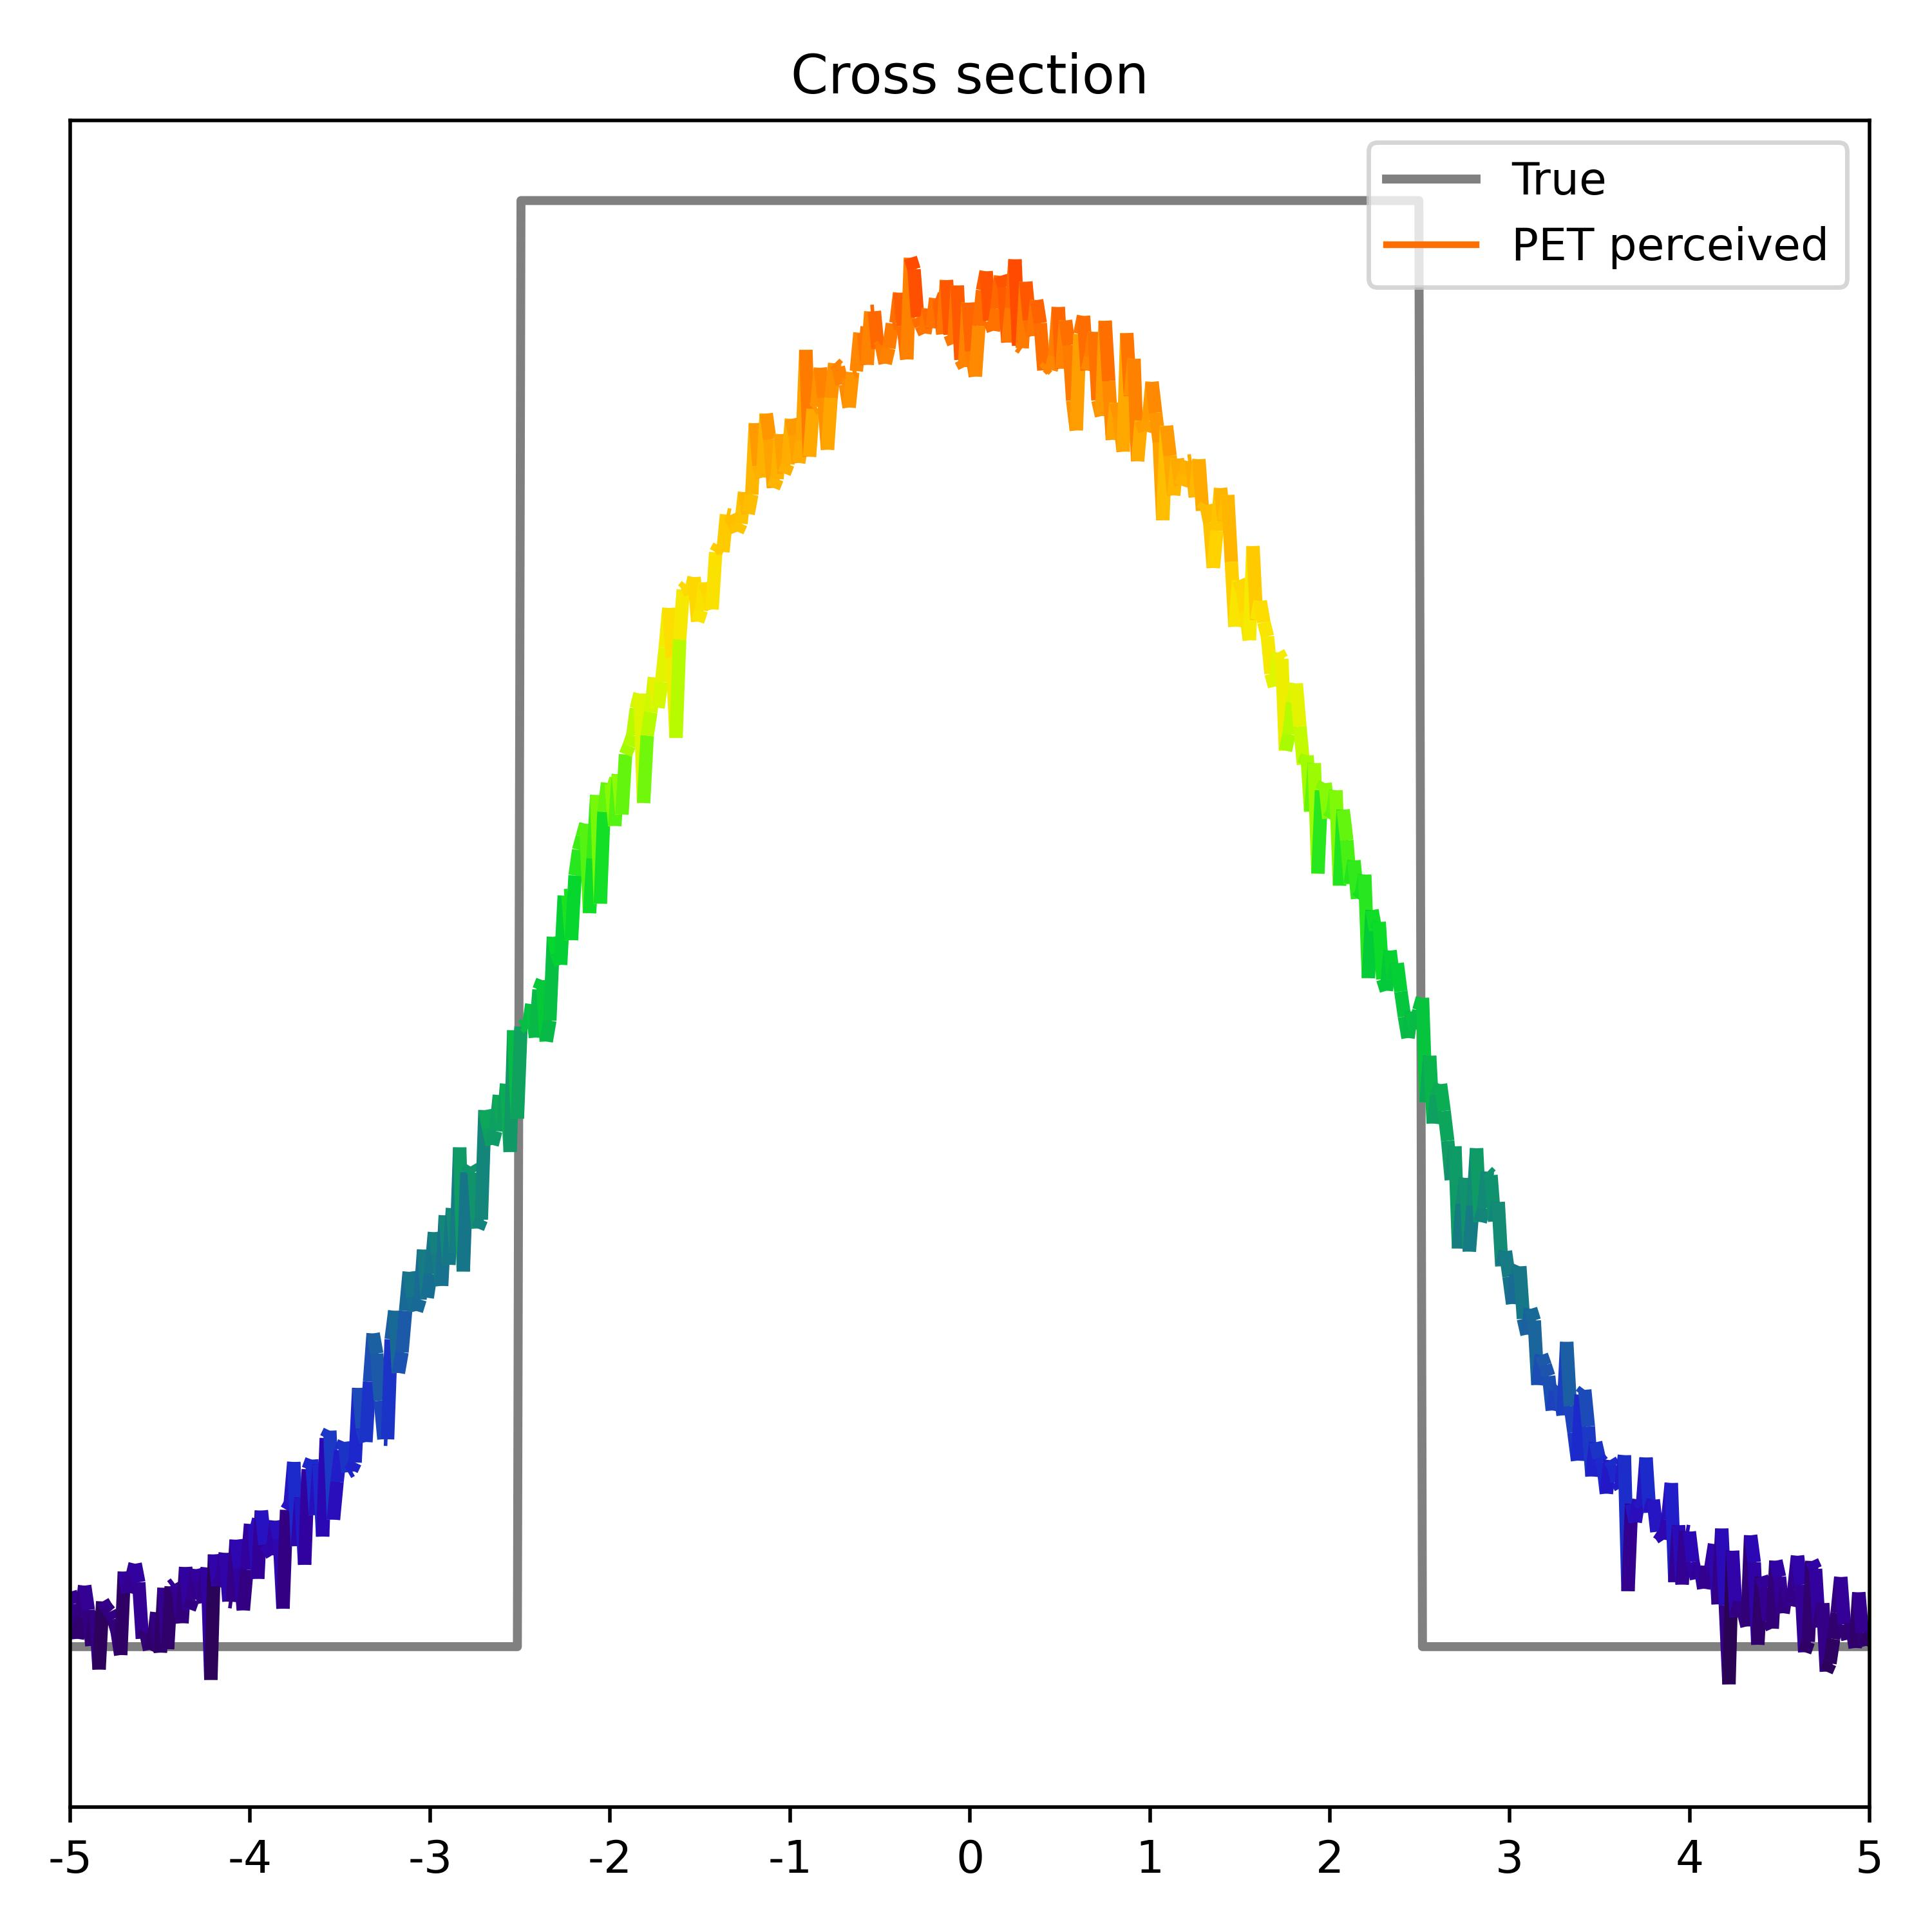
\includegraphics[height=5cm]{pve_crosssection.jpg}
	\end{center}
\end{frame}


\begin{frame}[t]{Partial Volume Correction (PVC) Methods Methods}
	\begin{columns}
		\begin{column}{0.65\textwidth}
			\small
			\begin{itemize}
				\setlength\itemsep{2em}
				\item \textbf{\citeauthoryear{feng2015image}}: Recovery Coefficient (RC): Spillage coefficients derived from cylindrical phantoms
				\item \textbf{\citeauthoryear{rousset1998correction}}: Geometric Transfer Matrix (GTM)
				\item \textbf{\citeauthoryear{ferrante2024physically}}: Deep learning model
				\item ...
			\end{itemize}
			\vspace{7em}
		\end{column}

		\begin{column}{0.35\textwidth}
			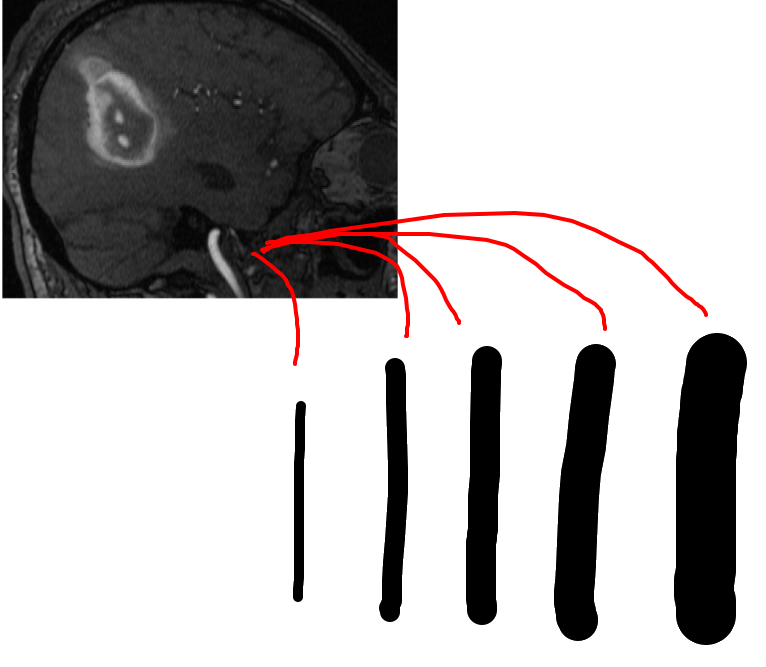
\includegraphics[width=0.8\linewidth]{/home/somso/thesis/rc.png}\par\vspace{1ex}

			% second image: wider than the column and shifted left to overlap the left column
			% tweak the two numbers below: the \hspace negative shift and the width of the image
			\makebox[0pt][l]{%
				\hspace{-1.2\textwidth}% <- how far left it intrudes (adjust)
				\includegraphics[width=1.8\textwidth]{/home/somso/thesis/deep.png}% <- actual displayed width (adjust)
			}

		\end{column}

	\end{columns}
\end{frame}


\begin{frame}[t]{Geometric Transfer Matrix (GTM)}
	\centering
	\begin{itemize}
		\setlength\itemsep{1em}
		\item Linear combination of the \textbf{true} Time Activity Curve (TAC) with \textbf{neighboring} regions
		\item Weights ($\omega_{x\rightarrow y}$) derived from modelling the effect of the Point Spread Function on geometry of regions
	\end{itemize}
	\vfill
	\begin{columns}
		\begin{column}{0.5\textwidth}
			\centering
			\begin{equation*}
				\underbrace{
					\begin{bmatrix}
						T_{c} \\
						T_{bg}
					\end{bmatrix}
				}_{\text{Observered}}
				=
				\underbrace{
					\begin{bmatrix}
						\omega_{c \rightarrow c}  & \omega_{bg \rightarrow c}  \\
						\omega_{c \rightarrow bg} & \omega_{bg \rightarrow bg}
					\end{bmatrix}
				}_{\text{GTM}}
				.
				\underbrace{
					\begin{bmatrix}
						T_{IF} \\
						T_{tissue}
					\end{bmatrix}
				}_{\text{Unknown}}
			\end{equation*}
		\end{column}
		\begin{column}{0.5\textwidth}
			\centering
			\begin{tikzpicture}
				\node[anchor=north west, inner sep=0] (img)
				at (0,0) {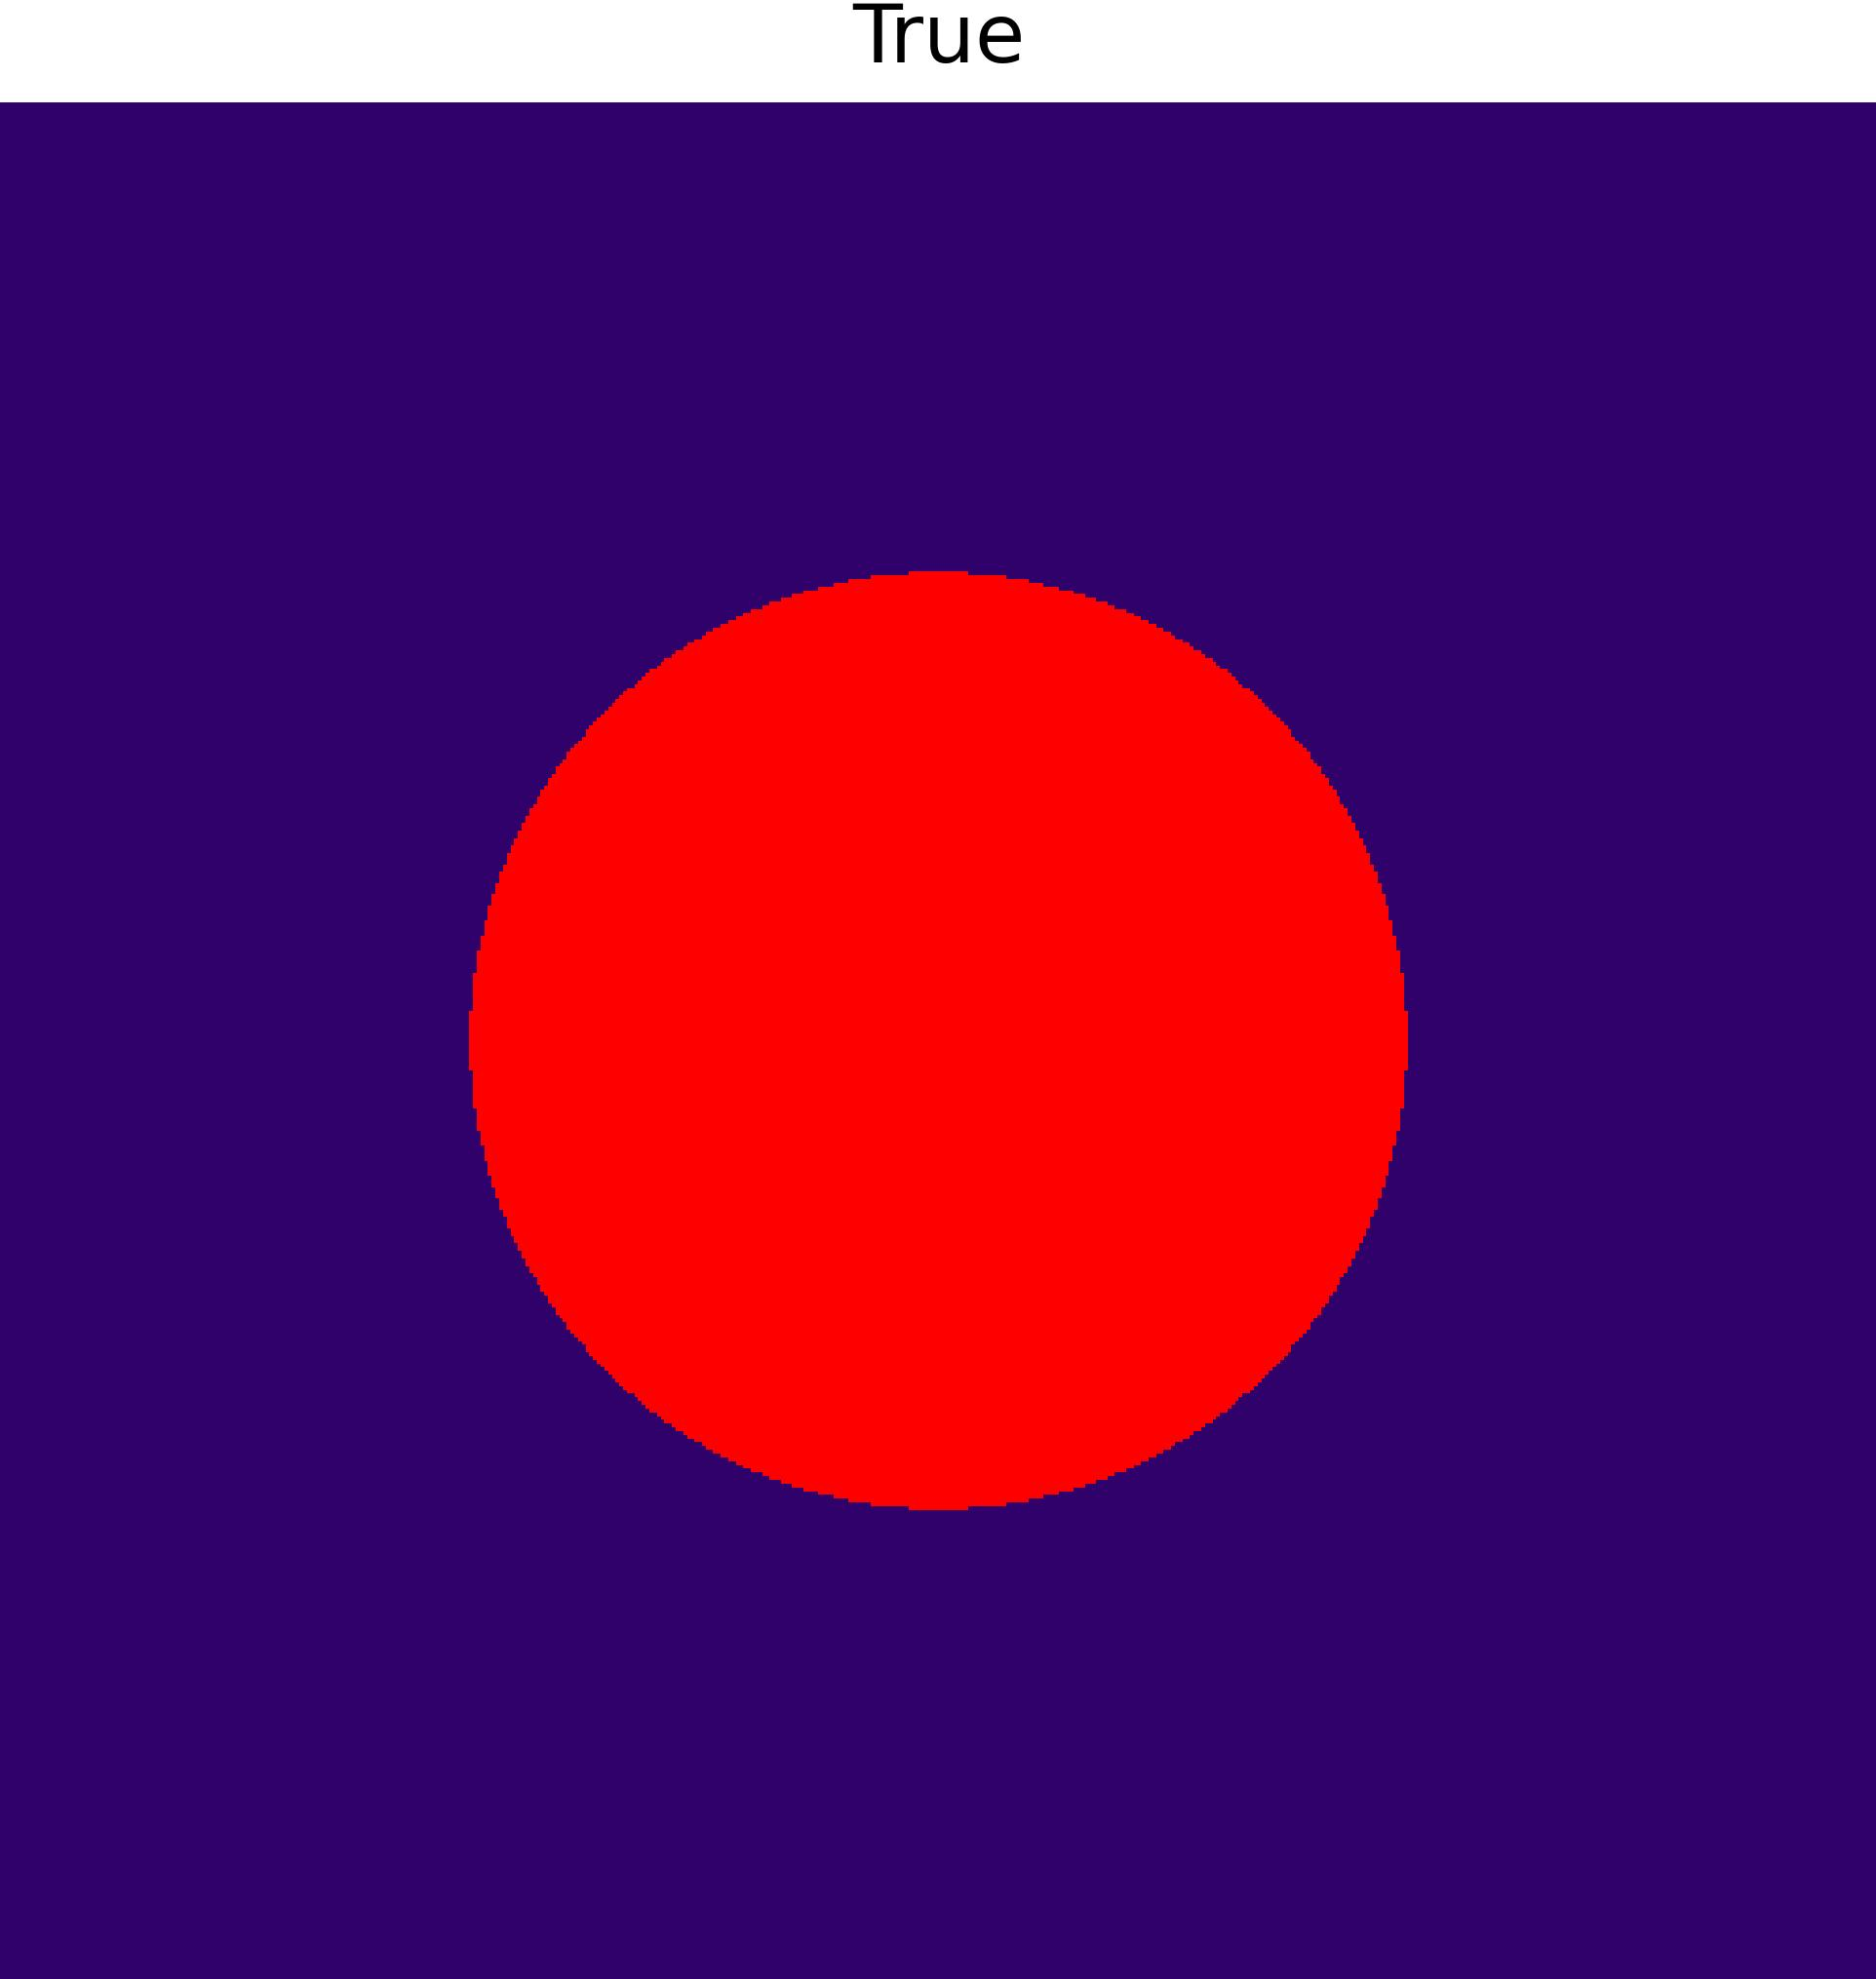
\includegraphics[height=4.5cm]{pve_true.jpg}};
				\begin{scope}[x={(img.north east)}, y={(img.south west)},visible on=<1->]
					\node[text=white, font=\scriptsize\bfseries] at (0.5,0.52) {Carotid};
					\node[text=white, font=\scriptsize\bfseries, anchor=west] at (0.8,0.52) {BG};

					\def\cx{0.50}
					\def\cy{0.50}
					\def\cr{0.25}

					% \draw[->, >=stealth, thick, white]
					% (\cx-\cr*0.25,\cy+\cr*0.65)
					% .. controls (\cx,\cy+\cr*0.90) and (\cx+\cr*0.35,\cy+\cr*0.65) ..
					% (\cx+\cr*0.15,\cy+\cr*0.30)
					% node[midway, below, text=white, font=\scriptsize] {$\omega_{c \rightarrow c}$};

					\draw[->, >=stealth, bend left=40,thick, color=white]
					(0.6,0.47) to node[above, text=white] {\small $\omega_{c\rightarrow bg}$} (0.85,0.48);

					\draw[<-, >=stealth, bend right=40,thick, color=white]
					(0.6,0.57) to node[below, text=white] {\small $\omega_{bg \rightarrow c}$} (0.85,0.56);
				\end{scope}
			\end{tikzpicture}

		\end{column}
	\end{columns}

	% 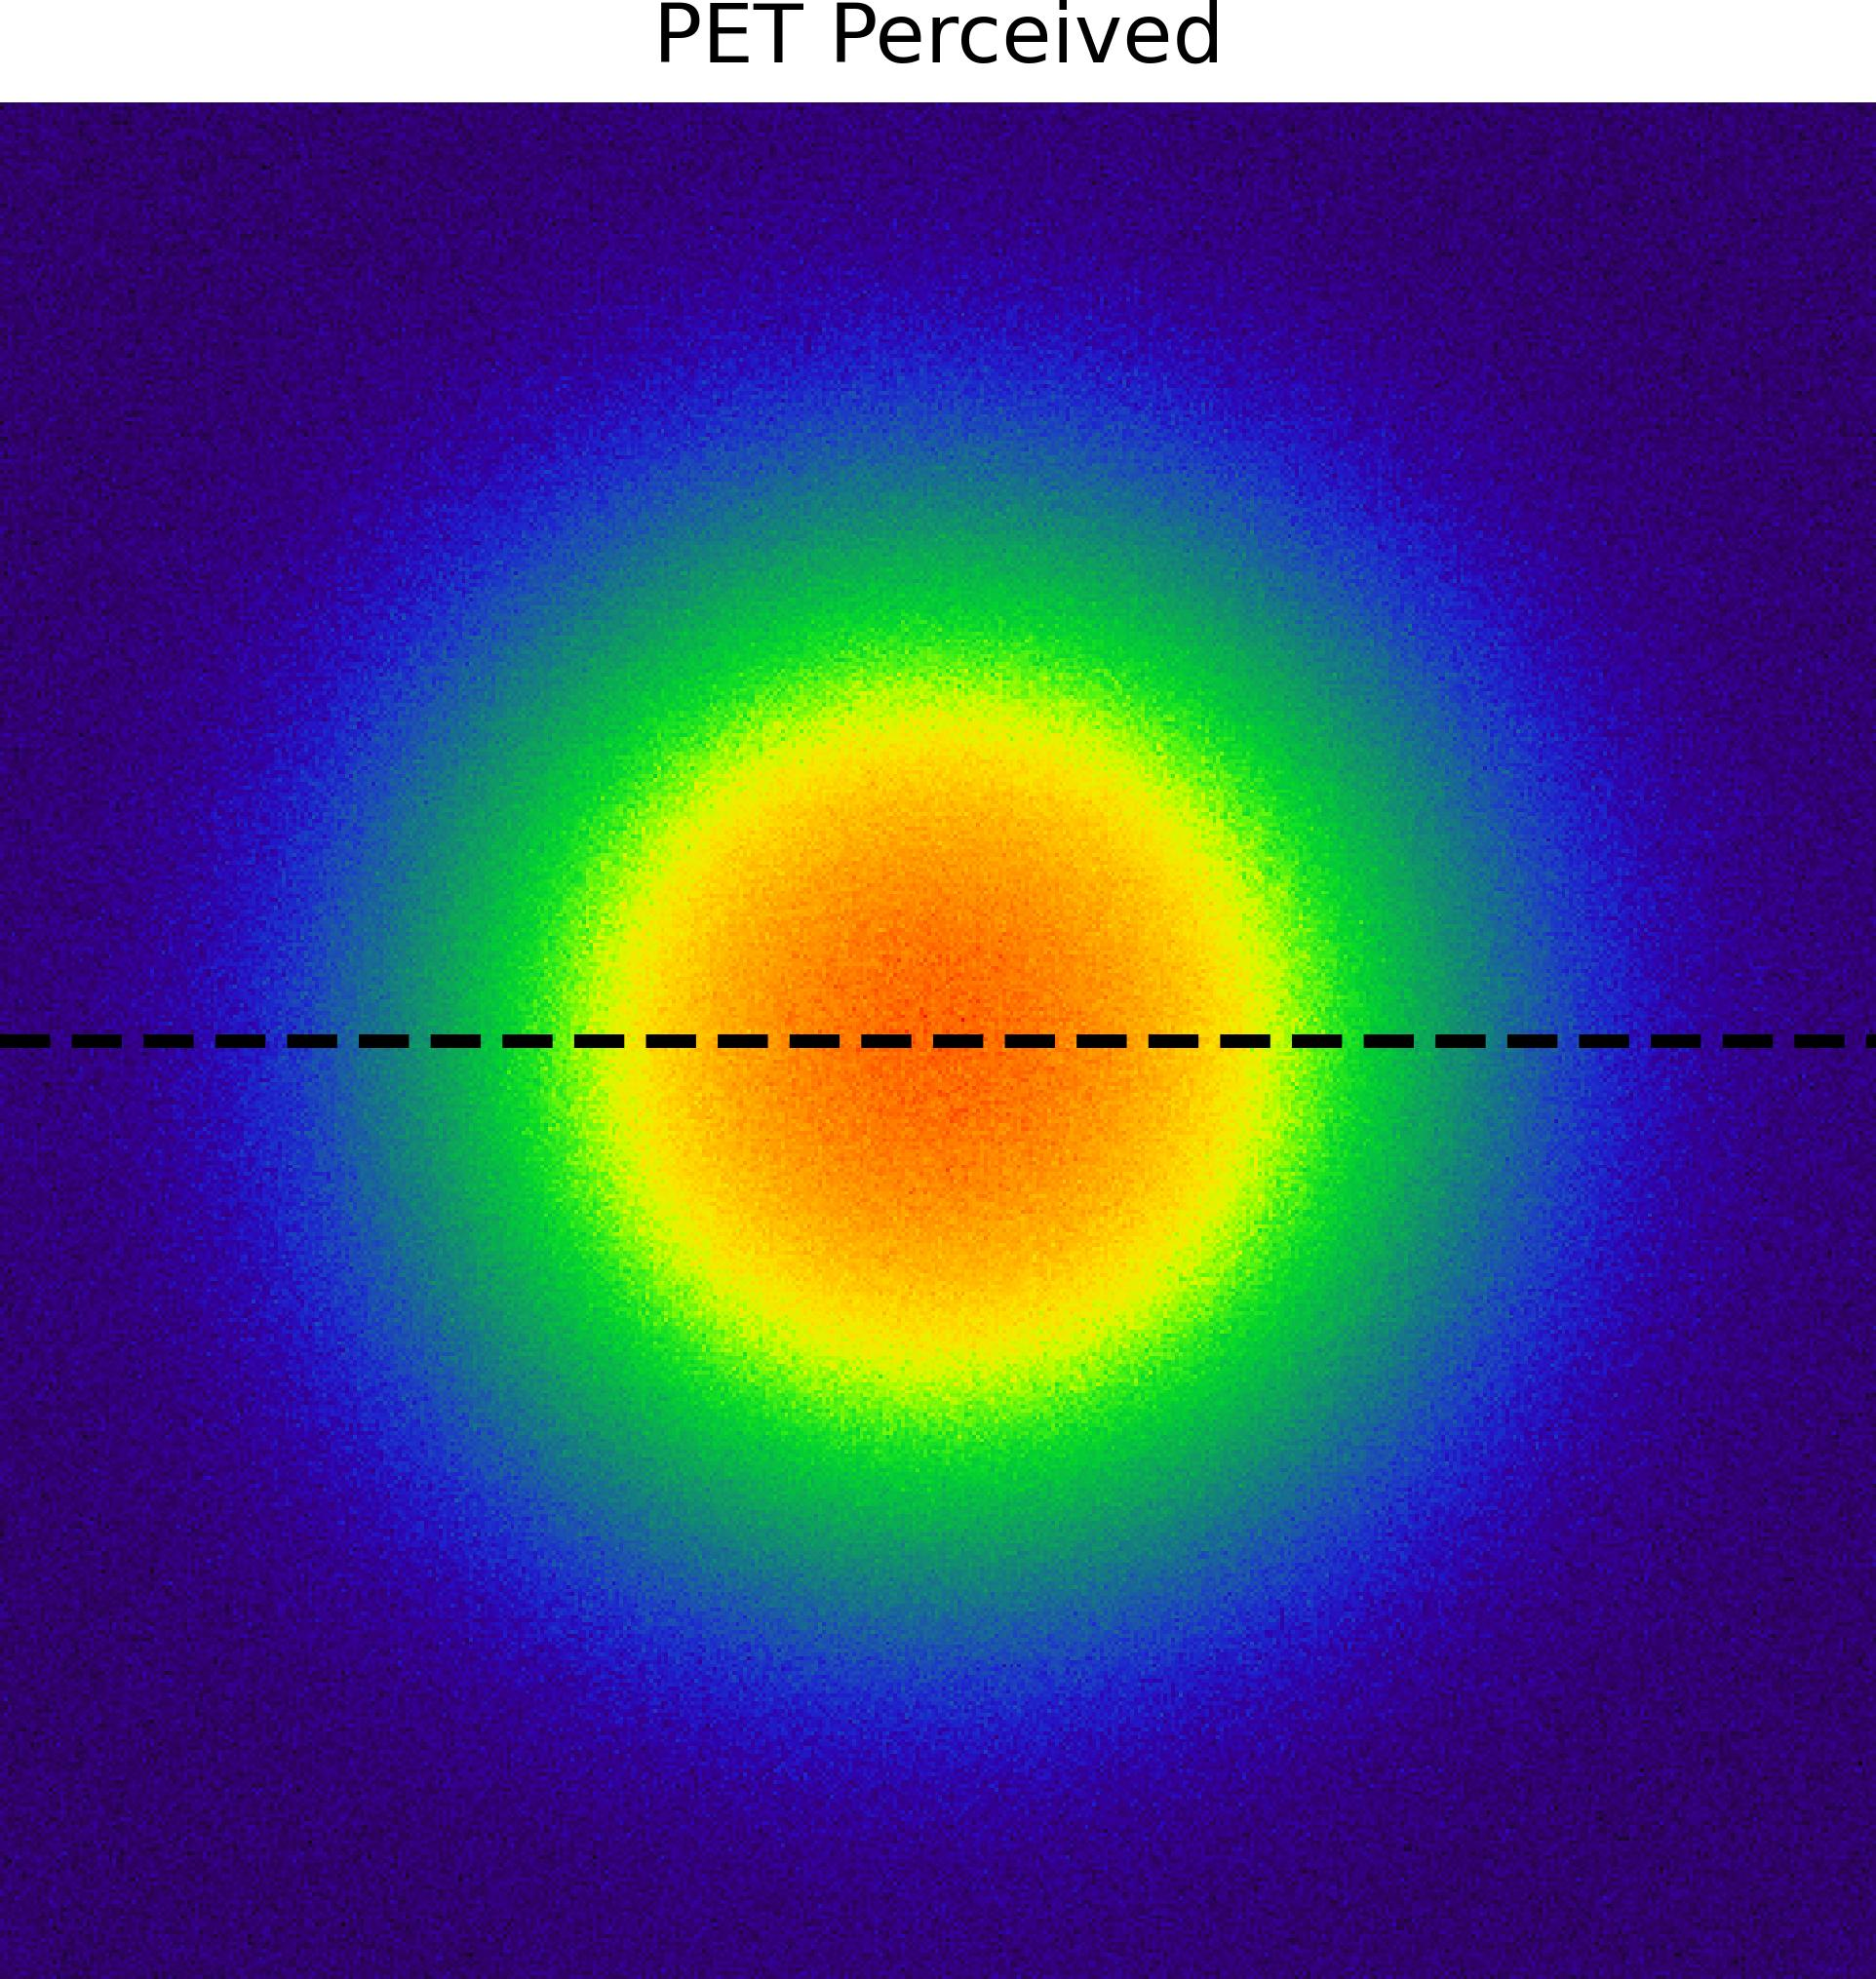
\includegraphics[height=4.5cm]{pve_perceived.jpg}
\end{frame}

\begin{frame}[t]{Geometric Transfer Matrix (GTM)}
	\centering
	\begin{center}
		% \begin{tikzpicture}
		% \end{tikzpicture}
		% 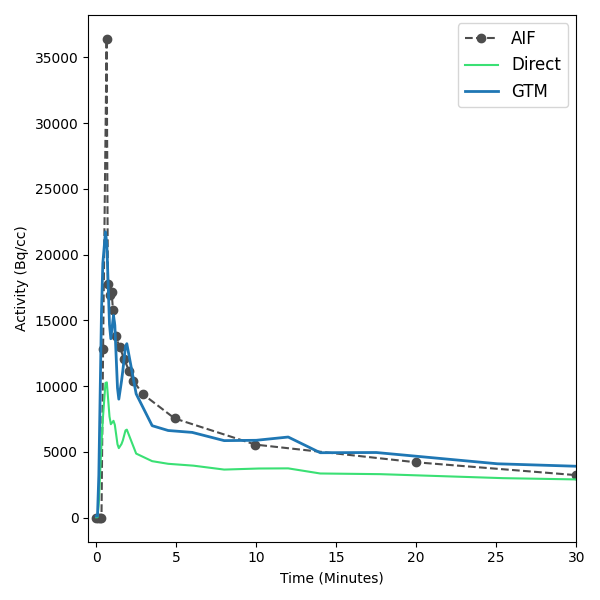
\includegraphics[height=6cm]{BADKA07504_1_bg_fg3.png}
		\begin{tikzpicture}
			\node[inner sep=0] (imgA) at (0,0)
			{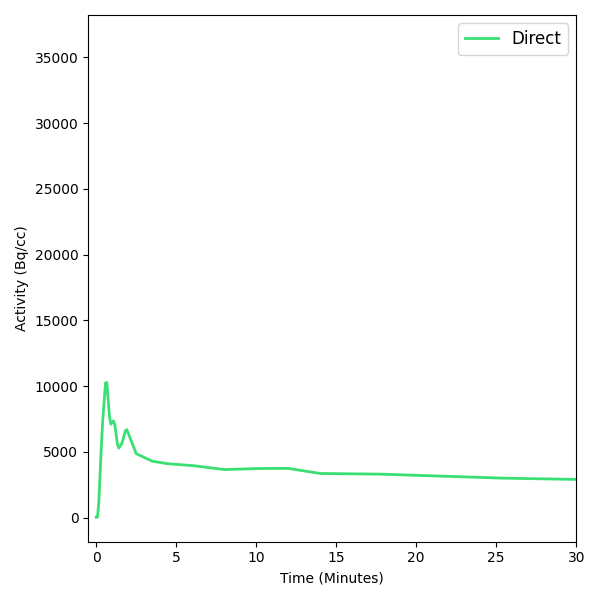
\includegraphics[height=5cm]{BADKA07504_1_bg_fg.png}};
			\node[above=0cm of imgA]{$\quad$Carotid};
			% Second image node to the right of the first (adjust xshift if you need spacing)
			\node[inner sep=0, right=0cm of imgA] (img)
			{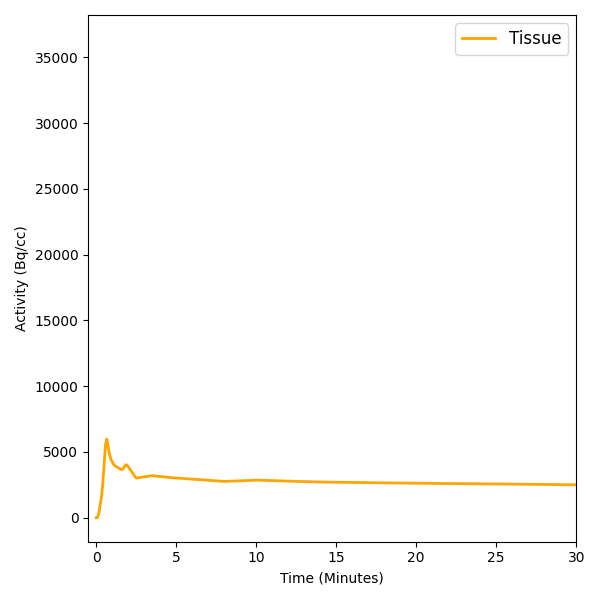
\includegraphics[height=5cm]{BADKA07504_1_bg_fg2.png}};
			\node[above=0cm of img]{$\quad$Surroundings};

			\node[inner sep=0, right=0cm of img,visible on=<2->] (imgC)
			{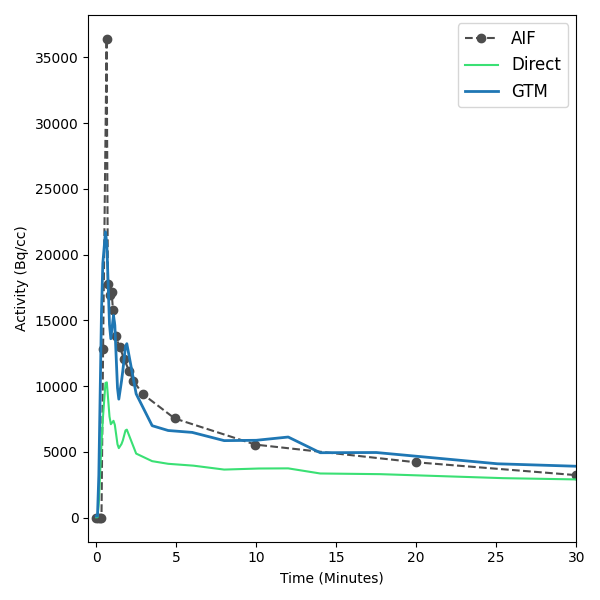
\includegraphics[height=5cm]{BADKA07504_1_bg_fg3.png}};
			\node[above=0cm of imgC,visible on=<2->]{$\quad$GTM Corrected};


			\draw[->, >=stealth, bend left=30,thick]
			(1.7,2.5) to node[above] {$\omega_{out}$} (3.5,2.5);

			\draw[<-, >=stealth, bend right=30,thick]
			(1.7,-2.5) to node[below] {\small $\omega_{in}$} (3.5,-2.5);
		\end{tikzpicture}


		\uncover<2->{\Large\textbf{Still not Accurate! The Noise is Amplified!}}
	\end{center}
\end{frame}

\begin{frame}{Objective}
	\centering\Large

	To replace the Invasive AIF:\\Obtain an accurate \textbf{segmentation} of the \textbf{carotids} from \textbf{MR-Angiography} for Image-Derived Input Function\\
	% \pause
	\bigskip
	+ \\
	\bigskip
	\Large{Develop a robust model to accurately account for \\
		\textbf{Partial Volume Effect (PVE)} and \textbf{Noise}}
\end{frame}

\begin{frame}{Modelling}
	\small
	\begin{block}{Input Function}
		\begin{itemize}
			\item Principal Component Analysis(PCA):
		\end{itemize}

		\[
			T_{IF}(t) = \mu_{IF}(t) +  \textcolor{red}{\theta_1}\,v_1(t) +  \textcolor{red}{\theta_2}\,v_2(t) +  \textcolor{red}{\theta_3}\,v_3(t)
		\]
		\(\mu_{IF}(t)\): Population mean AIF ($N$ Random subjects from the dataset)\\
		\(v_{i}(t)\): Principal components \\
		\(\theta_{i}\): Weighting coefficients
		% \vspace{3em}
	\end{block}
	\pause
	\begin{block}{Surrounding Tissue (The background)}
		\vspace{4pt}
		\begin{columns}[T]
			\begin{column}[T]{0.6\textwidth}
				\begin{itemize}
					\item
					      Spectral Analysis:
				\end{itemize}
				\vspace{1ex}
				\[
					T_{tissue}(t) = T_{IF} \circledast \textcolor{red}{\alpha}\,e^{-\textcolor{red}{\beta}t} (t)
				\]
				\\
				$\alpha$: Amplitude\\
				$\beta$: Decay Rate
			\end{column}

			\begin{column}{0.25\textwidth}
				\includegraphics[width=\linewidth]{/home/somso/thesis/sa.png}
			\end{column}
		\end{columns}
	\end{block}
\end{frame}

\begin{frame}{Modelling}
	\begin{block}{Noise}
		\begin{itemize}
			\setlength\itemsep{1.5em}
			\item Noise in PET is considered as a \textbf{Gaussian distribution}
			\item Noise level is not constant, rather It's \textbf{time-varying}
			\item It is summarized by a weighted average variance:
		\end{itemize}
		\[
			\sigma^2 = \frac{1}{N} \sum_{i=1}^{N} \omega_i\,\sigma_i^2.
		\]
		\(\omega_i\): Weighting Coefficient of frame $i$\\[1.5em]
		\(\sigma_i^2\): Variance of frame $i$\\[1.5em]
		$N$: Number of frames
		% \vspace{3em}
	\end{block}
\end{frame}



\begin{frame}[t]{Bayesian GTM (BGTM)}
	\begin{block}{Summary}
		\[
			\text{IF}(t) = \mathcal{F}(\textcolor{red}{\theta_1,\theta_2,\theta_3};t),
			\quad \text{BG}(t)=\mathcal{T}(\textcolor{red}{\alpha,\beta};t),
			\quad Noise=\textcolor{red}{\sigma^2}
		\]
		\[
			\text{IF} \xleftrightarrow{\text{\quad GTM\quad}} \text{BG}
		\]
	\end{block}
	\pause
	\begin{block}{Bayesian Parameter Estimation [\citeauthoryear{irace2021bayesian}]}
		\small
		\begin{itemize}
			\item<2-> Given observed PET data $\mathcal{D}$, estimate $\Theta=(\textcolor{red}{\theta_1, \theta_2, \theta_3, \alpha, \beta,\sigma^2})$
			\item<3-> Bayesian Estimation: Exploration using a Markov Chain Monte-Carlo Sampler:
			      \[
				      \underbrace{p(\Theta \mid \mathcal{D})}_{\text{Posterior}} \propto \underbrace{p(\mathcal{D} \mid \Theta)}_{\text{Likelihood}} \times \underbrace{\pi(\Theta)}_{\text{Prior}}
			      \]
			\item<4-> Choose the $\Theta$ with the highest posterior:
			      \[
				      \hat{\Theta} = \arg\max_{\Theta} \left\{ p(\Theta \mid \mathcal{D}) \right\}
				      \xrightarrow{\text{Best Solution}}
				      \textcolor{OliveGreen}{\text{IF} = \mathcal{F}(\hat{\theta}_1, \hat{\theta}_2, \hat{\theta}_3)}
			      \]
		\end{itemize}
	\end{block}
\end{frame}



\begin{frame}{Evaluation}
	\large{\textbf{Datasets:}}
	\begin{itemize}
		\setlength\itemsep{1.5em}
		% \large
		\item \fdg\ study: 59 comatose patients
		\item \yohimbine\ study: 7 healthy men
	\end{itemize}
	\vspace{1em}
	\large{\textbf{Evaluation Steps:}}
	\begin{enumerate}
		% \large
		\setlength\itemsep{1em}
		\item Segmentation: Visual inspection
		\item Input Function Curves: cumulative Area under the Curve (cAUC) comparison
		\item Regional Brain Absolute Quantification
		      \vspace{1ex}
		      \begin{itemize}
			      \setlength\itemsep{1em}
			      \item \fdg : Metabolic Rate of Glucose ($\mrglu$)
			      \item \yohimbine : Volume of Distribution ($V_T$)
		      \end{itemize}
	\end{enumerate}
\end{frame}

\section{Results}

\begin{frame}[t]{For a Specific \fdg\ Subject}
	\includegraphics[width=\textwidth]{/home/somso/thesis/scripts/ppca20_8/figures/estimation/input_function/BADKA07504_1_infunc.png}

\end{frame}

\begin{frame}[t]{For a Specific \fdg\ Subject}
	\begin{center}
		\vfill
		\begin{minipage}{0.48\textwidth}
			\centering
			\textbf{cAUC}
			\includegraphics[width=\linewidth]{/home/somso/thesis/scripts/ppca20_8/figures/estimation/input_function/BARPH08187_1_cauc.png}
		\end{minipage}
		\begin{minipage}{0.48\textwidth}
			\centering
			\textbf{Regional Quantification}
			\includegraphics[width=\linewidth]{/home/somso/thesis/scripts/ppca20_8/figures/quantification/BARPH08187_1_patlak_mrglu.png}
		\end{minipage}
		\vfill
	\end{center}
\end{frame}


\begin{frame}[t]{\fdg\ Overall Performance}
	\centering

	\begin{center}
		\begin{minipage}{0.35\textwidth}
			\centering
			\textbf{cAUC MAE}\\[0.5ex]
			\includegraphics[width=\linewidth]{/home/somso/thesis/scripts/ppca20_8/curve_mae_boxplot.png}
		\end{minipage}
		\hspace{2em}
		\begin{minipage}{0.35\textwidth}
			\centering
			\textbf{$\mrglu$ MAPE Quantification}\\[0.5ex]
			\includegraphics[width=\linewidth]{/home/somso/thesis/scripts/ppca20_8/quantification_patlak_mape_boxplot.png}
		\end{minipage}
	\end{center}
	{
	\small
	\begin{tabular}{l|ccc}
		\toprule
		Metric             & BGTM   & GTM    & PBIF   \\
		\midrule
		IF cAUC MAE        & 13,024 & 15,709 & 14,630 \\
		$\mrglu$ MAPE (\%) & 13\%   & 24\%   & 17\%   \\
		\bottomrule
	\end{tabular}
	}
\end{frame}

\begin{frame}[t]{\yohimbine\ Overall Performance}
	\centering

	\begin{center}
		\begin{minipage}{0.35\textwidth}
			\centering
			\textbf{cAUC MAE}\\[0.5ex]
			\includegraphics[width=\textwidth]{/home/somso/thesis/scripts/laur_1/curve_mae_boxplot.png}
		\end{minipage}
		\hspace{2em}
		\begin{minipage}{0.35\textwidth}
			\centering
			\textbf{$V_T$ MAPE Quantification}\\[0.5ex]
			\includegraphics[width=\textwidth]{/home/somso/thesis/scripts/laur_1/quantification_logan_mape_boxplot.png}
		\end{minipage}
	\end{center}

	{
	\small
	\begin{tabular}{l|ccc}
		\toprule
		Metric          & BGTM   & GTM    & PBIF   \\
		\midrule
		IF cAUC MAE     & 55,499 & 96,300 & 37,600 \\
		$V_T$ MAPE (\%) & 76\%   & 166\%  & 29\%   \\
		\bottomrule
	\end{tabular}

	}
\end{frame}

\begin{frame}{The Big Question}
	\centering \huge{Is the Arterial Blood Sampling Actually \\the Ground Truth?}
	\pause
	\vspace{1em} \\
	\large{Simulations can answer this by running experiments\\ in a controlled setting.}
\end{frame}

\begin{frame}{Simulation Design Pipeline}
	\resizebox{1.0\textwidth}{!}{%
		\begin{tikzpicture}[
				node distance=1cm and 2cm,
				auto,
				>=Stealth,
				mybox/.style={draw, rounded corners, rectangle, minimum width=2cm, minimum height=1cm, align=center}
			]

			\node[mybox,minimum width=3cm] (pet) {PET};
			\node[mybox,minimum width=3cm, below=of pet] (t1) {T1w MRI};
			\node[anchor=south east] at($(pet.north)+(0,0.5)$) (pet_image) {\includegraphics[height=2cm]{real_pet.png}};
			\node[right=0.1cm of pet_image] (t1_image) {\includegraphics[height=2cm]{t1.png}};


			\node[mybox, right=3cm of pet, minimum width=3cm] (ttac) {Tissue Activity};
			\node[mybox, right=3cm of t1, minimum width=3cm] (phantom) {Pseudo-realistic\\Phantom};

			\node[anchor=south east] at($(ttac.north)+(0,0.5)$) (phantom_image) {\includegraphics[height=2cm]{phantom.png}};
			\node[right=0cm of phantom_image] (ttac_image) {\includegraphics[height=2cm]{ttacs.png}};

			\node[mybox, right=1.5cm of ttac, minimum width=3.3cm] (proto) {Simulation \\ Description Protocol};
			\node[above=0.5cm of proto] (phantom_image) {\includegraphics[height=2cm]{simulation_input_pet.png}};

			% \node[mybox, right=2.2cm of proto, minimum width=3cm] (simpet) {Simulated PET};
			% \node[above=0.5cm of simpet] (phantom_image) {\includegraphics[height=2cm]{simulated_pet.png}};

			\draw[->]
			(pet.east) to[out=0, in=180]
			node[yshift=+2pt, above] {\scriptsize\textit{Compartmental}}
			node[yshift=-2pt, below] {\scriptsize\textit{Fitting \& PVC}}
			(ttac.west);

			\draw[->]
			(t1.east) to[out=0, in=180]
			node[yshift=+2pt, above] {\scriptsize\textit{Tissue}}
			node[yshift=-2pt, below] {\scriptsize\textit{Classification}}
			(phantom.west);

			\draw[->] (ttac.east) to[out=0, in=180] (proto.west);

			\draw[->] (phantom.east) to[out=0, in=180] (proto.west);

			% \draw[->]
			% (proto.east) to[out=0, in=180]
			% node[yshift=+2pt, above] {\textit{Monte Carlo}}
			% node[yshift=-2pt, below] {\textit{Simulation}}
			% (simpet.west);

			\begin{pgfonlayer}{background}
				\draw[dashed, rounded corners, thick]
				($(pet.north west)+(-0.3,0.3)$) rectangle ($(t1.south east)+(0.3,-0.3)$);
			\end{pgfonlayer}
			\node at ($(t1.south)-(0,0.6)$) {\text{Real Life Data}};
			\node at ($(t1.south)-(0,1.1)$) {\text{(\fdg\ Dataset)}};

			\begin{pgfonlayer}{background}
				\draw[dashed, rounded corners, thick]
				($(ttac.north west)+(-0.3,0.3)$) rectangle ($(phantom.south east)+(0.3,-0.3)$);
			\end{pgfonlayer}
			\node at ($(phantom.south)-(0,0.6)$) {\text{Ground Truth}};
		\end{tikzpicture}
		%
	}
\end{frame}

\begin{frame}{Simulation Results}
	\includegraphics[width=\textwidth]{sim_compare2.jpg}

\end{frame}

\begin{frame}[t]{Simulation Overall Performance}
	\centering
	\begin{center}
		\begin{minipage}{0.35\textwidth}
			\centering
			\textbf{cAUC MAE}\\[0.5ex]
			\includegraphics[width=\textwidth]{/home/somso/thesis/scripts/sim_18_7/curve_mae_boxplot.png}
		\end{minipage}
		\hspace{2em}
		\begin{minipage}{0.35\textwidth}
			\centering
			\textbf{$\mrglu$ MAPE Quantification}\\[0.5ex]
			\includegraphics[width=\textwidth]{/home/somso/thesis/scripts/sim_18_7/quantification_patlak_mape_boxplot.png}
		\end{minipage}
	\end{center}
	{
	\small
	\begin{tabular}{l|ccc}
		\toprule
		Metric             & BGTM   & GTM    & PBIF   \\
		\midrule
		IF cAUC MAE        & 53,997 & 57,991 & 23,072 \\
		$\mrglu$ MAPE (\%) & 48\%   & 35\%   & 18\%   \\
		\bottomrule
	\end{tabular}

	}
\end{frame}
\begin{frame}{Limitations \& Discussion}
	\begin{itemize}
		\setlength\itemsep{1.8em}
		\item Carotid segmentation relied on visual inspection can be further validated by \textbf{expert labels}
		\item Segmentation was designed for TOF-MRA and could be adapted to \textbf{T1} MRI
		\item \yohimbine\ suffered from \textbf{small PCA population}($N=6$) and subject \textbf{motion}
		\item Simulations showed \textbf{large bias} compared to the experimental dataset. Hinting to a faulty simulation design
		\item A more accurate \textbf{noise model} and \textbf{prior knowledge} can be explored
		      % \item The true source of discrepancy in the simulation is not known and needs further research
		      % \item Simulation design for IDIF proved to be \textbf{challenging and complex} and requires further research
		      % \item BGTM successfully recovers IDIF by jointly modelling PVE, Input Function, tissue, and noise
		      % \item Segmentation algorithm was simple yet fast and fully automatic
	\end{itemize}
\end{frame}

\begin{frame}{Conclusions}
	\begin{itemize}
		\setlength\itemsep{1.7em}
		\item In conclusion, BGTM successfully estimates an image-derived input function by jointly modelling \textbf{PVE, input function, tissue kinetics, and noise}
		\item BGTM showed \textbf{encouraging performance} on the \fdg\ cohort despite the challenging comatose cohort
		\item Segmentation algorithm was simple yet \textbf{fast and fully automatic}
		\item Simulation design proved to be challenging and needs further research
		\item Accurate simulations confirm \textbf{AIF} and also show \textbf{pitfalls} of IDIF estimation
		\item No assumptions were taken to allow for \textbf{generalizability} of the method
	\end{itemize}
\end{frame}

\begin{frame}[t,noframenumbering,plain]{Bibliography}
    \tiny
    \printbibliography[heading=none]
\end{frame}

\begin{frame}[noframenumbering,plain]
	\centering \huge{Thank you. \\ Questions?}
\end{frame}
\appendix

% \backupbegin 
\begin{backup}{\fdg\ Dataset}
	\centering
	\resizebox{\textwidth}{!}{% 
		\begin{tabular}{l|cc|cc|cc|cc|cc}
			\toprule
			\multirow{2}{*}{\textbf{Metric}} & \multicolumn{2}{c|}{\textbf{BGTM}} & \multicolumn{2}{c|}{\textbf{GTM}} & \multicolumn{2}{c|}{\textbf{PBIF}} & \multicolumn{2}{c|}{\textbf{BGTM vs GTM}} & \multicolumn{2}{c}{\textbf{BGTM vs PBIF}}                                                                                                                  \\
			\cmidrule(lr){2-3} \cmidrule(lr){4-5} \cmidrule(lr){6-7} \cmidrule(lr){8-9} \cmidrule(lr){10-11}
			                                 & \(\mu\)                            & \(\sigma\)                        & \(\mu\)                            & \(\sigma\)                                & \(\mu\)                                   & \(\sigma\) & \(t\)      & \(p\)                              & \(t\)      & \(p\)                              \\
			\midrule
			IF cAUC MAE                      & 13{,}024                           & 10{,}410                          & 15{,}709                           & 7{,}884                                   & 14{,}630                                  & 10{,}268   & \(-2.388\) & \(2.023\times 10^{-2}\) \sym{*}    & \(-1.278\) & \(2.065\times 10^{-1}\)            \\
			IF cAUC RMSE                     & 20{,}293                           & 16{,}078                          & 23{,}380                           & 11{,}979                                  & 23{,}334                                  & 16{,}803   & \(-1.907\) & \(6.151\times 10^{-2}\) \sym{\dag} & \(-1.439\) & \(1.555\times 10^{-1}\)            \\
			IF AUC APE (\%)                  & 11.93                              & 10.76                             & 11.57                              & 11.50                                     & 14.34                                     & 11.08      & \(0.297\)  & \(7.674\times 10^{-1}\)            & \(-1.862\) & \(6.767\times 10^{-2}\) \sym{\dag} \\
			\midrule
			\(\mrglu\) MAPE (\%)             & 13.19                              & 10.57                             & 24.36                              & 13.68                                     & 17.17                                     & 12.41      & \(-5.459\) & \(1.042\times 10^{-6}\) \sym{***}  & \(-2.415\) & \(1.890\times 10^{-2}\) \sym{*}    \\
			\(\mrglu\) MAE                   & 1.04                               & 0.92                              & 1.98                               & 1.33                                      & 1.40                                      & 1.10       & \(-5.934\) & \(1.754\times 10^{-7}\) \sym{***}  & \(-2.974\) & \(4.275\times 10^{-3}\) \sym{**}   \\
			\(R^2\) APE (\%)                 & 1.76                               & 4.07                              & 4.13                               & 8.90                                      & 1.50                                      & 3.53       & \(-2.762\) & \(7.677\times 10^{-3}\) \sym{**}   & \(1.680\)  & \(9.832\times 10^{-2}\)            \\
			Slope APE (\%)                   & 11.28                              & 9.37                              & 17.05                              & 10.58                                     & 15.76                                     & 11.41      & \(-4.030\) & \(1.644\times 10^{-4}\) \sym{***}  & \(-3.036\) & \(3.583\times 10^{-3}\) \sym{**}   \\
			\bottomrule
		\end{tabular}
		%
	}
	\\[1cm]
	Significance codes: \sym{*}\,p<0.05, \sym{**}\,p<0.01, \sym{***}\,p<0.001, \sym{\dag}\,p<0.10

\end{backup}
\begin{backup}{\yohimbine\ Dataset}
	\centering
	\resizebox{\textwidth}{!}{%
		\begin{tabular}{l|cc|cc|cc|cc|cc}
			\toprule
			\multirow{2}{*}{\textbf{Metric}} & \multicolumn{2}{c|}{\textbf{BGTM}} & \multicolumn{2}{c|}{\textbf{GTM}} & \multicolumn{2}{c|}{\textbf{PBIF}} & \multicolumn{2}{c|}{\textbf{BGTM vs GTM}} & \multicolumn{2}{c}{\textbf{BGTM vs PBIF}}                                                                                                  \\
			\cmidrule(lr){2-3} \cmidrule(lr){4-5} \cmidrule(lr){6-7} \cmidrule(lr){8-9} \cmidrule(lr){10-11}
			                                 & \(\mu\)                            & \(\sigma\)                        & \(\mu\)                            & \(\sigma\)                                & \(\mu\)                                   & \(\sigma\) & \(t\)      & \(p\)                          & \(t\)      & \(p\)                  \\
			\midrule
			IF cAUC MAE                      & 55{,}499                           & 40{,}271                          & 96{,}362                           & 20{,}343                                  & 37{,}613                                  & 20{,}456   & \(-3.404\) & \(1.443\times10^{-2}\)\sym{*}  & \(0.959\)  & \(3.748\times10^{-1}\) \\
			IF cAUC RMSE                     & 83{,}282                           & 60{,}130                          & 147{,}032                          & 28{,}318                                  & 52{,}313                                  & 27{,}845   & \(-3.789\) & \(9.083\times10^{-3}\)\sym{**} & \(1.196\)  & \(2.768\times10^{-1}\) \\
			IF AUC APE (\%)                  & 26.14                              & 19.02                             & 52.75                              & 3.53                                      & 17.74                                     & 14.78      & \(-3.644\) & \(1.078\times10^{-2}\)\sym{*}  & \(0.872\)  & \(4.168\times10^{-1}\) \\
			\midrule
			\(V_T\) MAPE (\%)                & 75.91                              & 62.09                             & 166.48                             & 52.91                                     & 29.47                                     & 17.73      & \(-3.628\) & \(1.100\times10^{-2}\)\sym{*}  & \(2.588\)  & \(4.133\times10^{-2}\) \\
			\(V_T\) MAE                      & 0.324                              & 0.211                             & 0.812                              & 0.360                                     & 0.132                                     & 0.072      & \(-3.477\) & \(1.318\times10^{-2}\)\sym{*}  & \(3.042\)  & \(2.275\times10^{-2}\) \\
			\(R^2\) APE (\%)                 & 2.04                               & 1.83                              & 2.27                               & 3.09                                      & 2.06                                      & 2.40       & \(-0.148\) & \(8.870\times10^{-1}\)         & \(-0.040\) & \(9.692\times10^{-1}\) \\
			Slope APE (\%)                   & 81.18                              & 68.33                             & 161.80                             & 73.59                                     & 35.06                                     & 24.22      & \(-3.167\) & \(1.939\times10^{-2}\)\sym{*}  & \(2.409\)  & \(5.263\times10^{-2}\) \\
			\bottomrule
		\end{tabular}%
	}
	\\[1cm]
	Significance codes: \sym{*}\,p<0.05, \sym{**}\,p<0.01, \sym{***}\,p<0.001, \sym{\dag}\,p<0.10
\end{backup}

\begin{backup}{Simulated Dataset}
	\centering
	\resizebox{\textwidth}{!}{%
		\begin{tabular}{l|cc|cc|cc|cc|cc}
			\toprule
			\multirow{2}{*}{\textbf{Metric}} & \multicolumn{2}{c|}{\textbf{BGTM}} & \multicolumn{2}{c|}{\textbf{GTM}} & \multicolumn{2}{c|}{\textbf{PBIF}} & \multicolumn{2}{c|}{\textbf{BGTM vs GTM}} & \multicolumn{2}{c}{\textbf{BGTM vs PBIF}}                                                                                                 \\
			\cmidrule(lr){2-3} \cmidrule(lr){4-5} \cmidrule(lr){6-7} \cmidrule(lr){8-9} \cmidrule(lr){10-11}
			                                 & \(\mu\)                            & \(\sigma\)                        & \(\mu\)                            & \(\sigma\)                                & \(\mu\)                                   & \(\sigma\) & \(t\)      & \(p\)                         & \(t\)     & \(p\)                   \\
			\midrule
			IF cAUC MAE                      & 53{,}997                           & 21{,}653                          & 57{,}991                           & 20{,}621                                  & 23{,}072                                  & 19{,}136   & \(-1.353\) & \(1.849\times10^{-1}\)        & \(9.013\) & \(1.556\times10^{-10}\) \\
			IF cAUC RMSE                     & 71{,}835                           & 28{,}603                          & 79{,}860                           & 29{,}010                                  & 30{,}451                                  & 25{,}946   & \(-2.105\) & \(4.279\times10^{-2}\)\sym{*} & \(8.805\) & \(2.732\times10^{-10}\) \\
			IF AUC APE (\%)                  & 33.35                              & 9.20                              & 36.13                              & 9.46                                      & 12.94                                     & 10.59      & \(-1.612\) & \(1.162\times10^{-1}\)        & \(8.317\) & \(1.043\times10^{-9}\)  \\
			\midrule
			\(\mrglu\) MAPE (\%)             & 48.14                              & 27.09                             & 35.60                              & 22.39                                     & 18.56                                     & 11.58      & \(2.678\)  & \(1.133\times10^{-2}\)        & \(6.578\) & \(1.545\times10^{-7}\)  \\
			\(\mrglu\) MAE                   & 4.62                               & 2.13                              & 3.49                               & 2.21                                      & 1.82                                      & 1.08       & \(2.463\)  & \(1.901\times10^{-2}\)        & \(7.598\) & \(7.919\times10^{-9}\)  \\
			\(R^2\) APE (\%)                 & 0.35                               & 0.88                              & 0.65                               & 0.88                                      & 0.32                                      & 0.59       & \(-1.636\) & \(1.111\times10^{-1}\)        & \(0.609\) & \(5.466\times10^{-1}\)  \\
			Slope APE (\%)                   & 45.58                              & 23.70                             & 39.97                              & 23.74                                     & 16.86                                     & 11.37      & \(1.297\)  & \(2.035\times10^{-1}\)        & \(6.812\) & \(7.750\times10^{-8}\)  \\
			\bottomrule
		\end{tabular}% 
	}
	\\[1cm]
	Significance codes: \sym{*}\,p<0.05, \sym{**}\,p<0.01, \sym{***}\,p<0.001, \sym{\dag}\,p<0.10
\end{backup}


\begin{backup}{Comparison of relative temporal bias (\%) of Direct IDIF}
	\includegraphics[width=\textwidth]{figures/GM12051_temporal_error.png}
\end{backup}


\begin{backup}{PCA Tuning}
	\centering
	\includegraphics[width=\textwidth]{pca_explained_variance.jpg}
\end{backup}
\begin{backup}{PCA Tuning}
	\centering
	\includegraphics[width=0.76\textwidth]{pca_n_experiment.jpg}
\end{backup}

\begin{backup}[t]{Noise Weighting}
	\[
		\sigma^2 = \frac{1}{N} \sum_{i=1}^{N} \omega_i\,\sigma_i^2.
	\]
	% \(\omega_i\): Weighting Coefficient of frame $i$\\[0.9em]
	\(\sigma_i^2\): Variance of frame $i$\\[0.9em]
	$N$: Number of frames
	\[
		\omega_{i} = \frac{\Delta t_i}{c_i}\,\exp\!\left(-\frac{t_{i}\,\ln 2}{T_{1/2}}\right)
	\]
	\\
	$\Delta t_i$: Frame durations in seconds \\[0.9em]
	$c_i$: Net true counts \\[0.9em]
	$t_i$: Mid-time of the frame \\[0.9em]
	$T_{1/2}$: Radioisotope half-life
\end{backup}


\end{document}
